\documentclass[8pt,twocolumn]{article}
%\usepackage{amsmath,amssymb,amsthm,amsbsy,amsfonts,mathtools}
\usepackage{amsmath}
\usepackage{amssymb}
\usepackage{amsthm}
\usepackage{physics}
\usepackage{hyperref}
\usepackage{exercise}
\usepackage[makeroom]{cancel}
\usepackage[margin=2em]{geometry}

\usepackage{graphicx}

\usepackage{footmisc}
\DefineFNsymbols{mySymbols}{{\ensuremath\dagger}{\ensuremath\ddagger}\S\P
   *{**}{\ensuremath{\dagger\dagger}}{\ensuremath{\ddagger\ddagger}}}
\setfnsymbol{mySymbols}

\newcommand{\N}{\mathbb{N}}
\newcommand{\R}{\mathbb{R}}
\newcommand{\Z}{\mathbb{Z}}
\newcommand{\Q}{\mathbb{Q}}

\newenvironment{theorem}[2][Theorem]{\begin{trivlist}
\item[\hskip \labelsep {\bfseries #1}\hskip \labelsep {\bfseries #2.}]}{\end{trivlist}}
\newenvironment{lemma}[2][Lemma]{\begin{trivlist}
\item[\hskip \labelsep {\bfseries #1}\hskip \labelsep {\bfseries #2.}]}{\end{trivlist}}
\newenvironment{exercise}[2][Exercise]{\begin{trivlist}
\item[\hskip \labelsep {\bfseries #1}\hskip \labelsep {\bfseries #2.}]}{\end{trivlist}}
\newenvironment{problem}[2][Problem]{\begin{trivlist}
\item[\hskip \labelsep {\bfseries #1}\hskip \labelsep {\bfseries #2.}]}{\end{trivlist}}
\newenvironment{question}[2][Question]{\begin{trivlist}
\item[\hskip \labelsep {\bfseries #1}\hskip \labelsep {\bfseries #2.}]}{\end{trivlist}}
\newenvironment{corollary}[2][Corollary]{\begin{trivlist}
\item[\hskip \labelsep {\bfseries #1}\hskip \labelsep {\bfseries #2.}]}{\end{trivlist}}
\newenvironment{answer}[2][Answer]{\begin{trivlist}
\item[\hskip \labelsep {\bfseries #1}\hskip \labelsep {\bfseries #2.}]}{\end{trivlist}}

\let\emph\relax % there's no \RedeclareTextFontCommand
\DeclareTextFontCommand{\emph}{\bfseries\em}

\setlength{\columnseprule}{0.4pt}
\setlength{\columnsep}{3em}

\usepackage{todonotes}

\author{Yingbo Ma \thanks{Student ID: \tt{16058474}}}
\title{\vspace{-1.cm}Homework 5}
\date{May 15, 2018}

\begin{document}
\maketitle

\begin{Answer}[number=29]
  \emph{16.1.29:}
  The function $f(x,y) = x^2 + y^2$ has the gradient $\grad f(x,y) =
  \mqty[2x\\2y]$. All the vectors point away from the origin.
  Thus $\grad f$ corresponds to graph \RC3.

  \emph{16.1.30:}
  The function $f(x,y) = x(x+y)$ has the gradient $\grad f(x,y) =
  \mqty[2x+y\\x]$. The vectors point upward when $x>0$, and vectors point
  downward when $x<0$.
  Thus $\grad f$ corresponds to graph \RC4.

  \emph{16.1.31:}
  The function $f(x,y) = (x+y)^2$ has the gradient $\grad f(x,y) =
  \mqty[2x+2y\\2x+2y]$. The vectors vanish along the line $y=-x$.
  Thus $\grad f$ corresponds to graph \RC2.

  \emph{16.1.32:}
  The function $f(x,y) = \sin \sqrt{x^2+y^2}$ has the gradient $\grad f(x,y) =
  \frac{\cos\sqrt{x^2+y^2}}{\sqrt{x^2+y^2}}\mqty[x\\y]$. The magnitude of
  vectors changes periodically as its distance grows from the origin.
  Thus $\grad f$ corresponds to graph \RC1.

  \emph{16.2.17:}
  \begin{enumerate}
    \item
      The function $\bm{F}$ have positive $y$-component along the line $x=-3$, and
      since the path goes upward, the integrand of the integral
      $\int_{C_1}\bm{F}\cdot \dd{\bm{r}} = \int_{C_1}\bm{F}\cdot\bm{T} \dd{s}$ always
      stay positive, thus the line integral is also positive.
    \item
      The function $\bm{F}$ goes in a clockwise fashion, while the curve $C_2$
      goes counterclockwise, and they are opposite. Thus the value of the line
      integral must be negative.
  \end{enumerate}

  \emph{16.2.8:}
  Let $C = C1 + C2$ and we have $C_1: x=2\cos t, y=2\sin t, 0\le t \le
  \frac{\pi}{2}$ and $C_2: x=4t, y=t+2, 0\le t\le 1$. We then have the integral
  \begin{align*}
    \int_C x^2\dd{x}+y^2\dd{y} &= \int_{C_1} x^2\dd{x}+y^2\dd{y} + \int_{C_2}
    x^2\dd{x}+y^2\dd{y} \\
    &= \int_0^{\frac{\pi}{2}}(2\cos t)^2 (-2\sin t\dd{t}) \\
    &+ (2\sin t)^2 (2\cos t\dd{t}) + \int_0^1 (4t)^2 4\dd{t} + (t+2)^2 \dd{t}
    \\
    &= \int_0^{\frac{\pi}{2}}8 (\sin^2 t \cos t - \cos^2 t\sin t)\dd{t} \\
    &+\int_0^1 65t^2+4t+4 \dd{t}
  \end{align*}
\end{Answer}

\begin{Answer}[number=30]
  Let $f(x,y)=x^2y$ and let $\bm{F}(x,y)=\grad f(x,y) = \mqty[2xy\\ x^2]$. We
  have $C_1: x=2t, y=4t, 0\le t\le 1$ and $C_2: x=2t, y=4t^2, 0\le t\le 1$. We
  have
  \begin{align*}
    \int_{C_1} \bm{F}\cdot \dd{\bm{r}} &= \int_{C_1} 2xy \dd{x} + x^2\dd{y} \\
    &= \int_0^1 2(2t)(4t) 2\dd{t} + (4t)^2 4\dd{t} = 16\int_0^1 3t^2\dd{t} \\
    &=16 \eval{t^3}_0^1 = 16
  \end{align*}
  and
  \begin{align*}
    \int_{C_2} \bm{F}\cdot \dd{\bm{r}} &= \int_{C_2} 2xy \dd{x} + x^2\dd{y} \\
    &= \int_0^1 2(2t)(4t^2) 2\dd{t} + (2t^2)^2 8t\dd{t} = \int_0^1 32t^3 + 32t^3\dd{t} \\
    &= 16\int_0^1 4t^3 \dd{t} = 16 \eval{t^4}_0^1 = 18.
  \end{align*}
  Thus, \(\int_{C_2} \bm{F}\cdot \dd{\bm{r}}\) and \(\int_{C_1} \bm{F}\cdot
  \dd{\bm{r}}\) have the same value.
\end{Answer}

\begin{Answer}[number=31]
  \begin{itemize}
    \item
      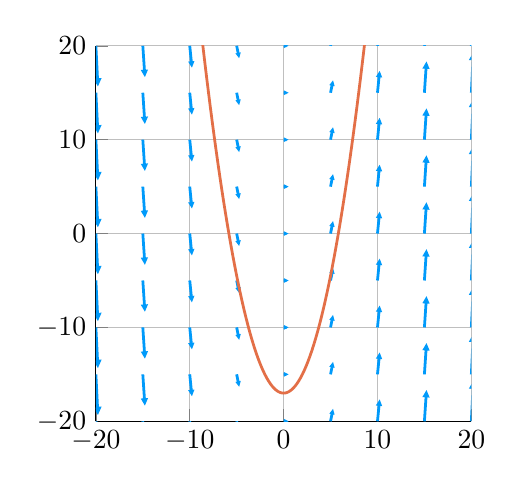
\begin{tikzpicture}[]
\begin{axis}[height = {63.5mm}, ylabel = {}, xmin = {-20.0}, xmax = {20.0}, ymax = {20.0}, xlabel = {}, unbounded coords=jump,scaled x ticks = false,xticklabel style={rotate = 0},xmajorgrids = true,xtick = {-20.0,-10.0,0.0,10.0,20.0},xticklabels = {$-20$,$-10$,$0$,$10$,$20$},xtick align = inside,axis lines* = left,scaled y ticks = false,yticklabel style={rotate = 0},ymajorgrids = true,ytick = {-20.0,-10.0,0.0,10.0,20.0},yticklabels = {$-20$,$-10$,$0$,$10$,$20$},ytick align = inside,axis lines* = left,    xshift = 0.0mm,
    yshift = 0.0mm,
    axis background/.style={fill={rgb,1:red,1.00000000;green,1.00000000;blue,1.00000000}}
, ymin = {-20.0}, width = {63.5mm}]\addplot+ [color = {rgb,1:red,0.00000000;green,0.60560316;blue,0.97868012},
draw opacity=1.0,
line width=1,
solid,mark = none,
mark size = 2.0,
mark options = {
    color = {rgb,1:red,0.00000000;green,0.00000000;blue,0.00000000}, draw opacity = 1.0,
    fill = {rgb,1:red,0.00000000;green,0.60560316;blue,0.97868012}, fill opacity = 1.0,
    line width = 1,
    rotate = 0,
    solid
},fill = {rgb,1:red,0.00000000;green,0.60560316;blue,0.97868012}, fill opacity=1.0,forget plot]coordinates {
(-20.0, -20.0)
(-19.82, -23.6)
(-19.62, -23.59)
(-19.8, -24.0)
(-20.02, -23.610000000000003)
(-19.82, -23.6)
};
\addplot+ [color = {rgb,1:red,0.00000000;green,0.60560316;blue,0.97868012},
draw opacity=1.0,
line width=1,
solid,mark = none,
mark size = 2.0,
mark options = {
    color = {rgb,1:red,0.00000000;green,0.00000000;blue,0.00000000}, draw opacity = 1.0,
    fill = {rgb,1:red,0.00000000;green,0.60560316;blue,0.97868012}, fill opacity = 1.0,
    line width = 1,
    rotate = 0,
    solid
},fill = {rgb,1:red,0.00000000;green,0.60560316;blue,0.97868012}, fill opacity=1.0,forget plot]coordinates {
(-15.0, -20.0)
(-14.82, -22.7)
(-14.67, -22.689999999999998)
(-14.8, -23.0)
(-14.97, -22.71)
(-14.82, -22.7)
};
\addplot+ [color = {rgb,1:red,0.00000000;green,0.60560316;blue,0.97868012},
draw opacity=1.0,
line width=1,
solid,mark = none,
mark size = 2.0,
mark options = {
    color = {rgb,1:red,0.00000000;green,0.00000000;blue,0.00000000}, draw opacity = 1.0,
    fill = {rgb,1:red,0.00000000;green,0.60560316;blue,0.97868012}, fill opacity = 1.0,
    line width = 1,
    rotate = 0,
    solid
},fill = {rgb,1:red,0.00000000;green,0.60560316;blue,0.97868012}, fill opacity=1.0,forget plot]coordinates {
(-10.0, -20.0)
(-9.82, -21.8)
(-9.72, -21.79)
(-9.8, -22.0)
(-9.92, -21.810000000000002)
(-9.82, -21.8)
};
\addplot+ [color = {rgb,1:red,0.00000000;green,0.60560316;blue,0.97868012},
draw opacity=1.0,
line width=1,
solid,mark = none,
mark size = 2.0,
mark options = {
    color = {rgb,1:red,0.00000000;green,0.00000000;blue,0.00000000}, draw opacity = 1.0,
    fill = {rgb,1:red,0.00000000;green,0.60560316;blue,0.97868012}, fill opacity = 1.0,
    line width = 1,
    rotate = 0,
    solid
},fill = {rgb,1:red,0.00000000;green,0.60560316;blue,0.97868012}, fill opacity=1.0,forget plot]coordinates {
(-5.0, -20.0)
(-4.819999999999999, -20.9)
(-4.77, -20.889999999999997)
(-4.8, -21.0)
(-4.869999999999999, -20.91)
(-4.819999999999999, -20.9)
};
\addplot+ [color = {rgb,1:red,0.00000000;green,0.60560316;blue,0.97868012},
draw opacity=1.0,
line width=1,
solid,mark = none,
mark size = 2.0,
mark options = {
    color = {rgb,1:red,0.00000000;green,0.00000000;blue,0.00000000}, draw opacity = 1.0,
    fill = {rgb,1:red,0.00000000;green,0.60560316;blue,0.97868012}, fill opacity = 1.0,
    line width = 1,
    rotate = 0,
    solid
},fill = {rgb,1:red,0.00000000;green,0.60560316;blue,0.97868012}, fill opacity=1.0,forget plot]coordinates {
(0.0, -20.0)
(0.18, -20.0)
(0.18, -19.99)
(0.2, -20.0)
(0.18, -20.01)
(0.18, -20.0)
};
\addplot+ [color = {rgb,1:red,0.00000000;green,0.60560316;blue,0.97868012},
draw opacity=1.0,
line width=1,
solid,mark = none,
mark size = 2.0,
mark options = {
    color = {rgb,1:red,0.00000000;green,0.00000000;blue,0.00000000}, draw opacity = 1.0,
    fill = {rgb,1:red,0.00000000;green,0.60560316;blue,0.97868012}, fill opacity = 1.0,
    line width = 1,
    rotate = 0,
    solid
},fill = {rgb,1:red,0.00000000;green,0.60560316;blue,0.97868012}, fill opacity=1.0,forget plot]coordinates {
(5.0, -20.0)
(5.180000000000001, -19.1)
(5.130000000000001, -19.09)
(5.2, -19.0)
(5.23, -19.110000000000003)
(5.180000000000001, -19.1)
};
\addplot+ [color = {rgb,1:red,0.00000000;green,0.60560316;blue,0.97868012},
draw opacity=1.0,
line width=1,
solid,mark = none,
mark size = 2.0,
mark options = {
    color = {rgb,1:red,0.00000000;green,0.00000000;blue,0.00000000}, draw opacity = 1.0,
    fill = {rgb,1:red,0.00000000;green,0.60560316;blue,0.97868012}, fill opacity = 1.0,
    line width = 1,
    rotate = 0,
    solid
},fill = {rgb,1:red,0.00000000;green,0.60560316;blue,0.97868012}, fill opacity=1.0,forget plot]coordinates {
(10.0, -20.0)
(10.18, -18.2)
(10.08, -18.189999999999998)
(10.2, -18.0)
(10.28, -18.21)
(10.18, -18.2)
};
\addplot+ [color = {rgb,1:red,0.00000000;green,0.60560316;blue,0.97868012},
draw opacity=1.0,
line width=1,
solid,mark = none,
mark size = 2.0,
mark options = {
    color = {rgb,1:red,0.00000000;green,0.00000000;blue,0.00000000}, draw opacity = 1.0,
    fill = {rgb,1:red,0.00000000;green,0.60560316;blue,0.97868012}, fill opacity = 1.0,
    line width = 1,
    rotate = 0,
    solid
},fill = {rgb,1:red,0.00000000;green,0.60560316;blue,0.97868012}, fill opacity=1.0,forget plot]coordinates {
(15.0, -20.0)
(15.18, -17.3)
(15.03, -17.29)
(15.2, -17.0)
(15.33, -17.310000000000002)
(15.18, -17.3)
};
\addplot+ [color = {rgb,1:red,0.00000000;green,0.60560316;blue,0.97868012},
draw opacity=1.0,
line width=1,
solid,mark = none,
mark size = 2.0,
mark options = {
    color = {rgb,1:red,0.00000000;green,0.00000000;blue,0.00000000}, draw opacity = 1.0,
    fill = {rgb,1:red,0.00000000;green,0.60560316;blue,0.97868012}, fill opacity = 1.0,
    line width = 1,
    rotate = 0,
    solid
},fill = {rgb,1:red,0.00000000;green,0.60560316;blue,0.97868012}, fill opacity=1.0,forget plot]coordinates {
(20.0, -20.0)
(20.18, -16.4)
(19.98, -16.389999999999997)
(20.2, -16.0)
(20.38, -16.41)
(20.18, -16.4)
};
\addplot+ [color = {rgb,1:red,0.00000000;green,0.60560316;blue,0.97868012},
draw opacity=1.0,
line width=1,
solid,mark = none,
mark size = 2.0,
mark options = {
    color = {rgb,1:red,0.00000000;green,0.00000000;blue,0.00000000}, draw opacity = 1.0,
    fill = {rgb,1:red,0.00000000;green,0.60560316;blue,0.97868012}, fill opacity = 1.0,
    line width = 1,
    rotate = 0,
    solid
},fill = {rgb,1:red,0.00000000;green,0.60560316;blue,0.97868012}, fill opacity=1.0,forget plot]coordinates {
(-20.0, -15.0)
(-19.82, -18.6)
(-19.62, -18.59)
(-19.8, -19.0)
(-20.02, -18.610000000000003)
(-19.82, -18.6)
};
\addplot+ [color = {rgb,1:red,0.00000000;green,0.60560316;blue,0.97868012},
draw opacity=1.0,
line width=1,
solid,mark = none,
mark size = 2.0,
mark options = {
    color = {rgb,1:red,0.00000000;green,0.00000000;blue,0.00000000}, draw opacity = 1.0,
    fill = {rgb,1:red,0.00000000;green,0.60560316;blue,0.97868012}, fill opacity = 1.0,
    line width = 1,
    rotate = 0,
    solid
},fill = {rgb,1:red,0.00000000;green,0.60560316;blue,0.97868012}, fill opacity=1.0,forget plot]coordinates {
(-15.0, -15.0)
(-14.82, -17.7)
(-14.67, -17.689999999999998)
(-14.8, -18.0)
(-14.97, -17.71)
(-14.82, -17.7)
};
\addplot+ [color = {rgb,1:red,0.00000000;green,0.60560316;blue,0.97868012},
draw opacity=1.0,
line width=1,
solid,mark = none,
mark size = 2.0,
mark options = {
    color = {rgb,1:red,0.00000000;green,0.00000000;blue,0.00000000}, draw opacity = 1.0,
    fill = {rgb,1:red,0.00000000;green,0.60560316;blue,0.97868012}, fill opacity = 1.0,
    line width = 1,
    rotate = 0,
    solid
},fill = {rgb,1:red,0.00000000;green,0.60560316;blue,0.97868012}, fill opacity=1.0,forget plot]coordinates {
(-10.0, -15.0)
(-9.82, -16.8)
(-9.72, -16.79)
(-9.8, -17.0)
(-9.92, -16.810000000000002)
(-9.82, -16.8)
};
\addplot+ [color = {rgb,1:red,0.00000000;green,0.60560316;blue,0.97868012},
draw opacity=1.0,
line width=1,
solid,mark = none,
mark size = 2.0,
mark options = {
    color = {rgb,1:red,0.00000000;green,0.00000000;blue,0.00000000}, draw opacity = 1.0,
    fill = {rgb,1:red,0.00000000;green,0.60560316;blue,0.97868012}, fill opacity = 1.0,
    line width = 1,
    rotate = 0,
    solid
},fill = {rgb,1:red,0.00000000;green,0.60560316;blue,0.97868012}, fill opacity=1.0,forget plot]coordinates {
(-5.0, -15.0)
(-4.819999999999999, -15.9)
(-4.77, -15.89)
(-4.8, -16.0)
(-4.869999999999999, -15.91)
(-4.819999999999999, -15.9)
};
\addplot+ [color = {rgb,1:red,0.00000000;green,0.60560316;blue,0.97868012},
draw opacity=1.0,
line width=1,
solid,mark = none,
mark size = 2.0,
mark options = {
    color = {rgb,1:red,0.00000000;green,0.00000000;blue,0.00000000}, draw opacity = 1.0,
    fill = {rgb,1:red,0.00000000;green,0.60560316;blue,0.97868012}, fill opacity = 1.0,
    line width = 1,
    rotate = 0,
    solid
},fill = {rgb,1:red,0.00000000;green,0.60560316;blue,0.97868012}, fill opacity=1.0,forget plot]coordinates {
(0.0, -15.0)
(0.18, -15.0)
(0.18, -14.99)
(0.2, -15.0)
(0.18, -15.01)
(0.18, -15.0)
};
\addplot+ [color = {rgb,1:red,0.00000000;green,0.60560316;blue,0.97868012},
draw opacity=1.0,
line width=1,
solid,mark = none,
mark size = 2.0,
mark options = {
    color = {rgb,1:red,0.00000000;green,0.00000000;blue,0.00000000}, draw opacity = 1.0,
    fill = {rgb,1:red,0.00000000;green,0.60560316;blue,0.97868012}, fill opacity = 1.0,
    line width = 1,
    rotate = 0,
    solid
},fill = {rgb,1:red,0.00000000;green,0.60560316;blue,0.97868012}, fill opacity=1.0,forget plot]coordinates {
(5.0, -15.0)
(5.180000000000001, -14.1)
(5.130000000000001, -14.09)
(5.2, -14.0)
(5.23, -14.11)
(5.180000000000001, -14.1)
};
\addplot+ [color = {rgb,1:red,0.00000000;green,0.60560316;blue,0.97868012},
draw opacity=1.0,
line width=1,
solid,mark = none,
mark size = 2.0,
mark options = {
    color = {rgb,1:red,0.00000000;green,0.00000000;blue,0.00000000}, draw opacity = 1.0,
    fill = {rgb,1:red,0.00000000;green,0.60560316;blue,0.97868012}, fill opacity = 1.0,
    line width = 1,
    rotate = 0,
    solid
},fill = {rgb,1:red,0.00000000;green,0.60560316;blue,0.97868012}, fill opacity=1.0,forget plot]coordinates {
(10.0, -15.0)
(10.18, -13.2)
(10.08, -13.19)
(10.2, -13.0)
(10.28, -13.209999999999999)
(10.18, -13.2)
};
\addplot+ [color = {rgb,1:red,0.00000000;green,0.60560316;blue,0.97868012},
draw opacity=1.0,
line width=1,
solid,mark = none,
mark size = 2.0,
mark options = {
    color = {rgb,1:red,0.00000000;green,0.00000000;blue,0.00000000}, draw opacity = 1.0,
    fill = {rgb,1:red,0.00000000;green,0.60560316;blue,0.97868012}, fill opacity = 1.0,
    line width = 1,
    rotate = 0,
    solid
},fill = {rgb,1:red,0.00000000;green,0.60560316;blue,0.97868012}, fill opacity=1.0,forget plot]coordinates {
(15.0, -15.0)
(15.18, -12.3)
(15.03, -12.290000000000001)
(15.2, -12.0)
(15.33, -12.31)
(15.18, -12.3)
};
\addplot+ [color = {rgb,1:red,0.00000000;green,0.60560316;blue,0.97868012},
draw opacity=1.0,
line width=1,
solid,mark = none,
mark size = 2.0,
mark options = {
    color = {rgb,1:red,0.00000000;green,0.00000000;blue,0.00000000}, draw opacity = 1.0,
    fill = {rgb,1:red,0.00000000;green,0.60560316;blue,0.97868012}, fill opacity = 1.0,
    line width = 1,
    rotate = 0,
    solid
},fill = {rgb,1:red,0.00000000;green,0.60560316;blue,0.97868012}, fill opacity=1.0,forget plot]coordinates {
(20.0, -15.0)
(20.18, -11.4)
(19.98, -11.39)
(20.2, -11.0)
(20.38, -11.41)
(20.18, -11.4)
};
\addplot+ [color = {rgb,1:red,0.00000000;green,0.60560316;blue,0.97868012},
draw opacity=1.0,
line width=1,
solid,mark = none,
mark size = 2.0,
mark options = {
    color = {rgb,1:red,0.00000000;green,0.00000000;blue,0.00000000}, draw opacity = 1.0,
    fill = {rgb,1:red,0.00000000;green,0.60560316;blue,0.97868012}, fill opacity = 1.0,
    line width = 1,
    rotate = 0,
    solid
},fill = {rgb,1:red,0.00000000;green,0.60560316;blue,0.97868012}, fill opacity=1.0,forget plot]coordinates {
(-20.0, -10.0)
(-19.82, -13.6)
(-19.62, -13.59)
(-19.8, -14.0)
(-20.02, -13.61)
(-19.82, -13.6)
};
\addplot+ [color = {rgb,1:red,0.00000000;green,0.60560316;blue,0.97868012},
draw opacity=1.0,
line width=1,
solid,mark = none,
mark size = 2.0,
mark options = {
    color = {rgb,1:red,0.00000000;green,0.00000000;blue,0.00000000}, draw opacity = 1.0,
    fill = {rgb,1:red,0.00000000;green,0.60560316;blue,0.97868012}, fill opacity = 1.0,
    line width = 1,
    rotate = 0,
    solid
},fill = {rgb,1:red,0.00000000;green,0.60560316;blue,0.97868012}, fill opacity=1.0,forget plot]coordinates {
(-15.0, -10.0)
(-14.82, -12.7)
(-14.67, -12.69)
(-14.8, -13.0)
(-14.97, -12.709999999999999)
(-14.82, -12.7)
};
\addplot+ [color = {rgb,1:red,0.00000000;green,0.60560316;blue,0.97868012},
draw opacity=1.0,
line width=1,
solid,mark = none,
mark size = 2.0,
mark options = {
    color = {rgb,1:red,0.00000000;green,0.00000000;blue,0.00000000}, draw opacity = 1.0,
    fill = {rgb,1:red,0.00000000;green,0.60560316;blue,0.97868012}, fill opacity = 1.0,
    line width = 1,
    rotate = 0,
    solid
},fill = {rgb,1:red,0.00000000;green,0.60560316;blue,0.97868012}, fill opacity=1.0,forget plot]coordinates {
(-10.0, -10.0)
(-9.82, -11.8)
(-9.72, -11.790000000000001)
(-9.8, -12.0)
(-9.92, -11.81)
(-9.82, -11.8)
};
\addplot+ [color = {rgb,1:red,0.00000000;green,0.60560316;blue,0.97868012},
draw opacity=1.0,
line width=1,
solid,mark = none,
mark size = 2.0,
mark options = {
    color = {rgb,1:red,0.00000000;green,0.00000000;blue,0.00000000}, draw opacity = 1.0,
    fill = {rgb,1:red,0.00000000;green,0.60560316;blue,0.97868012}, fill opacity = 1.0,
    line width = 1,
    rotate = 0,
    solid
},fill = {rgb,1:red,0.00000000;green,0.60560316;blue,0.97868012}, fill opacity=1.0,forget plot]coordinates {
(-5.0, -10.0)
(-4.819999999999999, -10.9)
(-4.77, -10.89)
(-4.8, -11.0)
(-4.869999999999999, -10.91)
(-4.819999999999999, -10.9)
};
\addplot+ [color = {rgb,1:red,0.00000000;green,0.60560316;blue,0.97868012},
draw opacity=1.0,
line width=1,
solid,mark = none,
mark size = 2.0,
mark options = {
    color = {rgb,1:red,0.00000000;green,0.00000000;blue,0.00000000}, draw opacity = 1.0,
    fill = {rgb,1:red,0.00000000;green,0.60560316;blue,0.97868012}, fill opacity = 1.0,
    line width = 1,
    rotate = 0,
    solid
},fill = {rgb,1:red,0.00000000;green,0.60560316;blue,0.97868012}, fill opacity=1.0,forget plot]coordinates {
(0.0, -10.0)
(0.18, -10.0)
(0.18, -9.99)
(0.2, -10.0)
(0.18, -10.01)
(0.18, -10.0)
};
\addplot+ [color = {rgb,1:red,0.00000000;green,0.60560316;blue,0.97868012},
draw opacity=1.0,
line width=1,
solid,mark = none,
mark size = 2.0,
mark options = {
    color = {rgb,1:red,0.00000000;green,0.00000000;blue,0.00000000}, draw opacity = 1.0,
    fill = {rgb,1:red,0.00000000;green,0.60560316;blue,0.97868012}, fill opacity = 1.0,
    line width = 1,
    rotate = 0,
    solid
},fill = {rgb,1:red,0.00000000;green,0.60560316;blue,0.97868012}, fill opacity=1.0,forget plot]coordinates {
(5.0, -10.0)
(5.180000000000001, -9.1)
(5.130000000000001, -9.09)
(5.2, -9.0)
(5.23, -9.11)
(5.180000000000001, -9.1)
};
\addplot+ [color = {rgb,1:red,0.00000000;green,0.60560316;blue,0.97868012},
draw opacity=1.0,
line width=1,
solid,mark = none,
mark size = 2.0,
mark options = {
    color = {rgb,1:red,0.00000000;green,0.00000000;blue,0.00000000}, draw opacity = 1.0,
    fill = {rgb,1:red,0.00000000;green,0.60560316;blue,0.97868012}, fill opacity = 1.0,
    line width = 1,
    rotate = 0,
    solid
},fill = {rgb,1:red,0.00000000;green,0.60560316;blue,0.97868012}, fill opacity=1.0,forget plot]coordinates {
(10.0, -10.0)
(10.18, -8.2)
(10.08, -8.19)
(10.2, -8.0)
(10.28, -8.209999999999999)
(10.18, -8.2)
};
\addplot+ [color = {rgb,1:red,0.00000000;green,0.60560316;blue,0.97868012},
draw opacity=1.0,
line width=1,
solid,mark = none,
mark size = 2.0,
mark options = {
    color = {rgb,1:red,0.00000000;green,0.00000000;blue,0.00000000}, draw opacity = 1.0,
    fill = {rgb,1:red,0.00000000;green,0.60560316;blue,0.97868012}, fill opacity = 1.0,
    line width = 1,
    rotate = 0,
    solid
},fill = {rgb,1:red,0.00000000;green,0.60560316;blue,0.97868012}, fill opacity=1.0,forget plot]coordinates {
(15.0, -10.0)
(15.18, -7.3)
(15.03, -7.29)
(15.2, -7.0)
(15.33, -7.31)
(15.18, -7.3)
};
\addplot+ [color = {rgb,1:red,0.00000000;green,0.60560316;blue,0.97868012},
draw opacity=1.0,
line width=1,
solid,mark = none,
mark size = 2.0,
mark options = {
    color = {rgb,1:red,0.00000000;green,0.00000000;blue,0.00000000}, draw opacity = 1.0,
    fill = {rgb,1:red,0.00000000;green,0.60560316;blue,0.97868012}, fill opacity = 1.0,
    line width = 1,
    rotate = 0,
    solid
},fill = {rgb,1:red,0.00000000;green,0.60560316;blue,0.97868012}, fill opacity=1.0,forget plot]coordinates {
(20.0, -10.0)
(20.18, -6.4)
(19.98, -6.390000000000001)
(20.2, -6.0)
(20.38, -6.41)
(20.18, -6.4)
};
\addplot+ [color = {rgb,1:red,0.00000000;green,0.60560316;blue,0.97868012},
draw opacity=1.0,
line width=1,
solid,mark = none,
mark size = 2.0,
mark options = {
    color = {rgb,1:red,0.00000000;green,0.00000000;blue,0.00000000}, draw opacity = 1.0,
    fill = {rgb,1:red,0.00000000;green,0.60560316;blue,0.97868012}, fill opacity = 1.0,
    line width = 1,
    rotate = 0,
    solid
},fill = {rgb,1:red,0.00000000;green,0.60560316;blue,0.97868012}, fill opacity=1.0,forget plot]coordinates {
(-20.0, -5.0)
(-19.82, -8.6)
(-19.62, -8.59)
(-19.8, -9.0)
(-20.02, -8.61)
(-19.82, -8.6)
};
\addplot+ [color = {rgb,1:red,0.00000000;green,0.60560316;blue,0.97868012},
draw opacity=1.0,
line width=1,
solid,mark = none,
mark size = 2.0,
mark options = {
    color = {rgb,1:red,0.00000000;green,0.00000000;blue,0.00000000}, draw opacity = 1.0,
    fill = {rgb,1:red,0.00000000;green,0.60560316;blue,0.97868012}, fill opacity = 1.0,
    line width = 1,
    rotate = 0,
    solid
},fill = {rgb,1:red,0.00000000;green,0.60560316;blue,0.97868012}, fill opacity=1.0,forget plot]coordinates {
(-15.0, -5.0)
(-14.82, -7.7)
(-14.67, -7.69)
(-14.8, -8.0)
(-14.97, -7.71)
(-14.82, -7.7)
};
\addplot+ [color = {rgb,1:red,0.00000000;green,0.60560316;blue,0.97868012},
draw opacity=1.0,
line width=1,
solid,mark = none,
mark size = 2.0,
mark options = {
    color = {rgb,1:red,0.00000000;green,0.00000000;blue,0.00000000}, draw opacity = 1.0,
    fill = {rgb,1:red,0.00000000;green,0.60560316;blue,0.97868012}, fill opacity = 1.0,
    line width = 1,
    rotate = 0,
    solid
},fill = {rgb,1:red,0.00000000;green,0.60560316;blue,0.97868012}, fill opacity=1.0,forget plot]coordinates {
(-10.0, -5.0)
(-9.82, -6.8)
(-9.72, -6.79)
(-9.8, -7.0)
(-9.92, -6.81)
(-9.82, -6.8)
};
\addplot+ [color = {rgb,1:red,0.00000000;green,0.60560316;blue,0.97868012},
draw opacity=1.0,
line width=1,
solid,mark = none,
mark size = 2.0,
mark options = {
    color = {rgb,1:red,0.00000000;green,0.00000000;blue,0.00000000}, draw opacity = 1.0,
    fill = {rgb,1:red,0.00000000;green,0.60560316;blue,0.97868012}, fill opacity = 1.0,
    line width = 1,
    rotate = 0,
    solid
},fill = {rgb,1:red,0.00000000;green,0.60560316;blue,0.97868012}, fill opacity=1.0,forget plot]coordinates {
(-5.0, -5.0)
(-4.819999999999999, -5.9)
(-4.77, -5.890000000000001)
(-4.8, -6.0)
(-4.869999999999999, -5.91)
(-4.819999999999999, -5.9)
};
\addplot+ [color = {rgb,1:red,0.00000000;green,0.60560316;blue,0.97868012},
draw opacity=1.0,
line width=1,
solid,mark = none,
mark size = 2.0,
mark options = {
    color = {rgb,1:red,0.00000000;green,0.00000000;blue,0.00000000}, draw opacity = 1.0,
    fill = {rgb,1:red,0.00000000;green,0.60560316;blue,0.97868012}, fill opacity = 1.0,
    line width = 1,
    rotate = 0,
    solid
},fill = {rgb,1:red,0.00000000;green,0.60560316;blue,0.97868012}, fill opacity=1.0,forget plot]coordinates {
(0.0, -5.0)
(0.18, -5.0)
(0.18, -4.99)
(0.2, -5.0)
(0.18, -5.01)
(0.18, -5.0)
};
\addplot+ [color = {rgb,1:red,0.00000000;green,0.60560316;blue,0.97868012},
draw opacity=1.0,
line width=1,
solid,mark = none,
mark size = 2.0,
mark options = {
    color = {rgb,1:red,0.00000000;green,0.00000000;blue,0.00000000}, draw opacity = 1.0,
    fill = {rgb,1:red,0.00000000;green,0.60560316;blue,0.97868012}, fill opacity = 1.0,
    line width = 1,
    rotate = 0,
    solid
},fill = {rgb,1:red,0.00000000;green,0.60560316;blue,0.97868012}, fill opacity=1.0,forget plot]coordinates {
(5.0, -5.0)
(5.180000000000001, -4.1)
(5.130000000000001, -4.09)
(5.2, -4.0)
(5.23, -4.109999999999999)
(5.180000000000001, -4.1)
};
\addplot+ [color = {rgb,1:red,0.00000000;green,0.60560316;blue,0.97868012},
draw opacity=1.0,
line width=1,
solid,mark = none,
mark size = 2.0,
mark options = {
    color = {rgb,1:red,0.00000000;green,0.00000000;blue,0.00000000}, draw opacity = 1.0,
    fill = {rgb,1:red,0.00000000;green,0.60560316;blue,0.97868012}, fill opacity = 1.0,
    line width = 1,
    rotate = 0,
    solid
},fill = {rgb,1:red,0.00000000;green,0.60560316;blue,0.97868012}, fill opacity=1.0,forget plot]coordinates {
(10.0, -5.0)
(10.18, -3.2)
(10.08, -3.1900000000000004)
(10.2, -3.0)
(10.28, -3.21)
(10.18, -3.2)
};
\addplot+ [color = {rgb,1:red,0.00000000;green,0.60560316;blue,0.97868012},
draw opacity=1.0,
line width=1,
solid,mark = none,
mark size = 2.0,
mark options = {
    color = {rgb,1:red,0.00000000;green,0.00000000;blue,0.00000000}, draw opacity = 1.0,
    fill = {rgb,1:red,0.00000000;green,0.60560316;blue,0.97868012}, fill opacity = 1.0,
    line width = 1,
    rotate = 0,
    solid
},fill = {rgb,1:red,0.00000000;green,0.60560316;blue,0.97868012}, fill opacity=1.0,forget plot]coordinates {
(15.0, -5.0)
(15.18, -2.3)
(15.03, -2.29)
(15.2, -2.0)
(15.33, -2.3099999999999996)
(15.18, -2.3)
};
\addplot+ [color = {rgb,1:red,0.00000000;green,0.60560316;blue,0.97868012},
draw opacity=1.0,
line width=1,
solid,mark = none,
mark size = 2.0,
mark options = {
    color = {rgb,1:red,0.00000000;green,0.00000000;blue,0.00000000}, draw opacity = 1.0,
    fill = {rgb,1:red,0.00000000;green,0.60560316;blue,0.97868012}, fill opacity = 1.0,
    line width = 1,
    rotate = 0,
    solid
},fill = {rgb,1:red,0.00000000;green,0.60560316;blue,0.97868012}, fill opacity=1.0,forget plot]coordinates {
(20.0, -5.0)
(20.18, -1.4000000000000001)
(19.98, -1.3900000000000001)
(20.2, -1.0)
(20.38, -1.4100000000000001)
(20.18, -1.4000000000000001)
};
\addplot+ [color = {rgb,1:red,0.00000000;green,0.60560316;blue,0.97868012},
draw opacity=1.0,
line width=1,
solid,mark = none,
mark size = 2.0,
mark options = {
    color = {rgb,1:red,0.00000000;green,0.00000000;blue,0.00000000}, draw opacity = 1.0,
    fill = {rgb,1:red,0.00000000;green,0.60560316;blue,0.97868012}, fill opacity = 1.0,
    line width = 1,
    rotate = 0,
    solid
},fill = {rgb,1:red,0.00000000;green,0.60560316;blue,0.97868012}, fill opacity=1.0,forget plot]coordinates {
(-20.0, 0.0)
(-19.82, -3.6)
(-19.62, -3.5900000000000003)
(-19.8, -4.0)
(-20.02, -3.61)
(-19.82, -3.6)
};
\addplot+ [color = {rgb,1:red,0.00000000;green,0.60560316;blue,0.97868012},
draw opacity=1.0,
line width=1,
solid,mark = none,
mark size = 2.0,
mark options = {
    color = {rgb,1:red,0.00000000;green,0.00000000;blue,0.00000000}, draw opacity = 1.0,
    fill = {rgb,1:red,0.00000000;green,0.60560316;blue,0.97868012}, fill opacity = 1.0,
    line width = 1,
    rotate = 0,
    solid
},fill = {rgb,1:red,0.00000000;green,0.60560316;blue,0.97868012}, fill opacity=1.0,forget plot]coordinates {
(-15.0, 0.0)
(-14.82, -2.7)
(-14.67, -2.6900000000000004)
(-14.8, -3.0)
(-14.97, -2.71)
(-14.82, -2.7)
};
\addplot+ [color = {rgb,1:red,0.00000000;green,0.60560316;blue,0.97868012},
draw opacity=1.0,
line width=1,
solid,mark = none,
mark size = 2.0,
mark options = {
    color = {rgb,1:red,0.00000000;green,0.00000000;blue,0.00000000}, draw opacity = 1.0,
    fill = {rgb,1:red,0.00000000;green,0.60560316;blue,0.97868012}, fill opacity = 1.0,
    line width = 1,
    rotate = 0,
    solid
},fill = {rgb,1:red,0.00000000;green,0.60560316;blue,0.97868012}, fill opacity=1.0,forget plot]coordinates {
(-10.0, 0.0)
(-9.82, -1.8)
(-9.72, -1.79)
(-9.8, -2.0)
(-9.92, -1.81)
(-9.82, -1.8)
};
\addplot+ [color = {rgb,1:red,0.00000000;green,0.60560316;blue,0.97868012},
draw opacity=1.0,
line width=1,
solid,mark = none,
mark size = 2.0,
mark options = {
    color = {rgb,1:red,0.00000000;green,0.00000000;blue,0.00000000}, draw opacity = 1.0,
    fill = {rgb,1:red,0.00000000;green,0.60560316;blue,0.97868012}, fill opacity = 1.0,
    line width = 1,
    rotate = 0,
    solid
},fill = {rgb,1:red,0.00000000;green,0.60560316;blue,0.97868012}, fill opacity=1.0,forget plot]coordinates {
(-5.0, 0.0)
(-4.819999999999999, -0.9)
(-4.77, -0.89)
(-4.8, -1.0)
(-4.869999999999999, -0.91)
(-4.819999999999999, -0.9)
};
\addplot+ [color = {rgb,1:red,0.00000000;green,0.60560316;blue,0.97868012},
draw opacity=1.0,
line width=1,
solid,mark = none,
mark size = 2.0,
mark options = {
    color = {rgb,1:red,0.00000000;green,0.00000000;blue,0.00000000}, draw opacity = 1.0,
    fill = {rgb,1:red,0.00000000;green,0.60560316;blue,0.97868012}, fill opacity = 1.0,
    line width = 1,
    rotate = 0,
    solid
},fill = {rgb,1:red,0.00000000;green,0.60560316;blue,0.97868012}, fill opacity=1.0,forget plot]coordinates {
(0.0, 0.0)
(0.18, 0.0)
(0.18, 0.010000000000000002)
(0.2, 0.0)
(0.18, -0.010000000000000002)
(0.18, 0.0)
};
\addplot+ [color = {rgb,1:red,0.00000000;green,0.60560316;blue,0.97868012},
draw opacity=1.0,
line width=1,
solid,mark = none,
mark size = 2.0,
mark options = {
    color = {rgb,1:red,0.00000000;green,0.00000000;blue,0.00000000}, draw opacity = 1.0,
    fill = {rgb,1:red,0.00000000;green,0.60560316;blue,0.97868012}, fill opacity = 1.0,
    line width = 1,
    rotate = 0,
    solid
},fill = {rgb,1:red,0.00000000;green,0.60560316;blue,0.97868012}, fill opacity=1.0,forget plot]coordinates {
(5.0, 0.0)
(5.180000000000001, 0.9)
(5.130000000000001, 0.91)
(5.2, 1.0)
(5.23, 0.89)
(5.180000000000001, 0.9)
};
\addplot+ [color = {rgb,1:red,0.00000000;green,0.60560316;blue,0.97868012},
draw opacity=1.0,
line width=1,
solid,mark = none,
mark size = 2.0,
mark options = {
    color = {rgb,1:red,0.00000000;green,0.00000000;blue,0.00000000}, draw opacity = 1.0,
    fill = {rgb,1:red,0.00000000;green,0.60560316;blue,0.97868012}, fill opacity = 1.0,
    line width = 1,
    rotate = 0,
    solid
},fill = {rgb,1:red,0.00000000;green,0.60560316;blue,0.97868012}, fill opacity=1.0,forget plot]coordinates {
(10.0, 0.0)
(10.18, 1.8)
(10.08, 1.81)
(10.2, 2.0)
(10.28, 1.79)
(10.18, 1.8)
};
\addplot+ [color = {rgb,1:red,0.00000000;green,0.60560316;blue,0.97868012},
draw opacity=1.0,
line width=1,
solid,mark = none,
mark size = 2.0,
mark options = {
    color = {rgb,1:red,0.00000000;green,0.00000000;blue,0.00000000}, draw opacity = 1.0,
    fill = {rgb,1:red,0.00000000;green,0.60560316;blue,0.97868012}, fill opacity = 1.0,
    line width = 1,
    rotate = 0,
    solid
},fill = {rgb,1:red,0.00000000;green,0.60560316;blue,0.97868012}, fill opacity=1.0,forget plot]coordinates {
(15.0, 0.0)
(15.18, 2.7)
(15.03, 2.71)
(15.2, 3.0)
(15.33, 2.6900000000000004)
(15.18, 2.7)
};
\addplot+ [color = {rgb,1:red,0.00000000;green,0.60560316;blue,0.97868012},
draw opacity=1.0,
line width=1,
solid,mark = none,
mark size = 2.0,
mark options = {
    color = {rgb,1:red,0.00000000;green,0.00000000;blue,0.00000000}, draw opacity = 1.0,
    fill = {rgb,1:red,0.00000000;green,0.60560316;blue,0.97868012}, fill opacity = 1.0,
    line width = 1,
    rotate = 0,
    solid
},fill = {rgb,1:red,0.00000000;green,0.60560316;blue,0.97868012}, fill opacity=1.0,forget plot]coordinates {
(20.0, 0.0)
(20.18, 3.6)
(19.98, 3.61)
(20.2, 4.0)
(20.38, 3.5900000000000003)
(20.18, 3.6)
};
\addplot+ [color = {rgb,1:red,0.00000000;green,0.60560316;blue,0.97868012},
draw opacity=1.0,
line width=1,
solid,mark = none,
mark size = 2.0,
mark options = {
    color = {rgb,1:red,0.00000000;green,0.00000000;blue,0.00000000}, draw opacity = 1.0,
    fill = {rgb,1:red,0.00000000;green,0.60560316;blue,0.97868012}, fill opacity = 1.0,
    line width = 1,
    rotate = 0,
    solid
},fill = {rgb,1:red,0.00000000;green,0.60560316;blue,0.97868012}, fill opacity=1.0,forget plot]coordinates {
(-20.0, 5.0)
(-19.82, 1.4000000000000001)
(-19.62, 1.4100000000000001)
(-19.8, 1.0)
(-20.02, 1.3900000000000001)
(-19.82, 1.4000000000000001)
};
\addplot+ [color = {rgb,1:red,0.00000000;green,0.60560316;blue,0.97868012},
draw opacity=1.0,
line width=1,
solid,mark = none,
mark size = 2.0,
mark options = {
    color = {rgb,1:red,0.00000000;green,0.00000000;blue,0.00000000}, draw opacity = 1.0,
    fill = {rgb,1:red,0.00000000;green,0.60560316;blue,0.97868012}, fill opacity = 1.0,
    line width = 1,
    rotate = 0,
    solid
},fill = {rgb,1:red,0.00000000;green,0.60560316;blue,0.97868012}, fill opacity=1.0,forget plot]coordinates {
(-15.0, 5.0)
(-14.82, 2.3)
(-14.67, 2.3099999999999996)
(-14.8, 2.0)
(-14.97, 2.29)
(-14.82, 2.3)
};
\addplot+ [color = {rgb,1:red,0.00000000;green,0.60560316;blue,0.97868012},
draw opacity=1.0,
line width=1,
solid,mark = none,
mark size = 2.0,
mark options = {
    color = {rgb,1:red,0.00000000;green,0.00000000;blue,0.00000000}, draw opacity = 1.0,
    fill = {rgb,1:red,0.00000000;green,0.60560316;blue,0.97868012}, fill opacity = 1.0,
    line width = 1,
    rotate = 0,
    solid
},fill = {rgb,1:red,0.00000000;green,0.60560316;blue,0.97868012}, fill opacity=1.0,forget plot]coordinates {
(-10.0, 5.0)
(-9.82, 3.2)
(-9.72, 3.21)
(-9.8, 3.0)
(-9.92, 3.1900000000000004)
(-9.82, 3.2)
};
\addplot+ [color = {rgb,1:red,0.00000000;green,0.60560316;blue,0.97868012},
draw opacity=1.0,
line width=1,
solid,mark = none,
mark size = 2.0,
mark options = {
    color = {rgb,1:red,0.00000000;green,0.00000000;blue,0.00000000}, draw opacity = 1.0,
    fill = {rgb,1:red,0.00000000;green,0.60560316;blue,0.97868012}, fill opacity = 1.0,
    line width = 1,
    rotate = 0,
    solid
},fill = {rgb,1:red,0.00000000;green,0.60560316;blue,0.97868012}, fill opacity=1.0,forget plot]coordinates {
(-5.0, 5.0)
(-4.819999999999999, 4.1)
(-4.77, 4.109999999999999)
(-4.8, 4.0)
(-4.869999999999999, 4.09)
(-4.819999999999999, 4.1)
};
\addplot+ [color = {rgb,1:red,0.00000000;green,0.60560316;blue,0.97868012},
draw opacity=1.0,
line width=1,
solid,mark = none,
mark size = 2.0,
mark options = {
    color = {rgb,1:red,0.00000000;green,0.00000000;blue,0.00000000}, draw opacity = 1.0,
    fill = {rgb,1:red,0.00000000;green,0.60560316;blue,0.97868012}, fill opacity = 1.0,
    line width = 1,
    rotate = 0,
    solid
},fill = {rgb,1:red,0.00000000;green,0.60560316;blue,0.97868012}, fill opacity=1.0,forget plot]coordinates {
(0.0, 5.0)
(0.18, 5.0)
(0.18, 5.01)
(0.2, 5.0)
(0.18, 4.99)
(0.18, 5.0)
};
\addplot+ [color = {rgb,1:red,0.00000000;green,0.60560316;blue,0.97868012},
draw opacity=1.0,
line width=1,
solid,mark = none,
mark size = 2.0,
mark options = {
    color = {rgb,1:red,0.00000000;green,0.00000000;blue,0.00000000}, draw opacity = 1.0,
    fill = {rgb,1:red,0.00000000;green,0.60560316;blue,0.97868012}, fill opacity = 1.0,
    line width = 1,
    rotate = 0,
    solid
},fill = {rgb,1:red,0.00000000;green,0.60560316;blue,0.97868012}, fill opacity=1.0,forget plot]coordinates {
(5.0, 5.0)
(5.180000000000001, 5.9)
(5.130000000000001, 5.91)
(5.2, 6.0)
(5.23, 5.890000000000001)
(5.180000000000001, 5.9)
};
\addplot+ [color = {rgb,1:red,0.00000000;green,0.60560316;blue,0.97868012},
draw opacity=1.0,
line width=1,
solid,mark = none,
mark size = 2.0,
mark options = {
    color = {rgb,1:red,0.00000000;green,0.00000000;blue,0.00000000}, draw opacity = 1.0,
    fill = {rgb,1:red,0.00000000;green,0.60560316;blue,0.97868012}, fill opacity = 1.0,
    line width = 1,
    rotate = 0,
    solid
},fill = {rgb,1:red,0.00000000;green,0.60560316;blue,0.97868012}, fill opacity=1.0,forget plot]coordinates {
(10.0, 5.0)
(10.18, 6.8)
(10.08, 6.81)
(10.2, 7.0)
(10.28, 6.79)
(10.18, 6.8)
};
\addplot+ [color = {rgb,1:red,0.00000000;green,0.60560316;blue,0.97868012},
draw opacity=1.0,
line width=1,
solid,mark = none,
mark size = 2.0,
mark options = {
    color = {rgb,1:red,0.00000000;green,0.00000000;blue,0.00000000}, draw opacity = 1.0,
    fill = {rgb,1:red,0.00000000;green,0.60560316;blue,0.97868012}, fill opacity = 1.0,
    line width = 1,
    rotate = 0,
    solid
},fill = {rgb,1:red,0.00000000;green,0.60560316;blue,0.97868012}, fill opacity=1.0,forget plot]coordinates {
(15.0, 5.0)
(15.18, 7.7)
(15.03, 7.71)
(15.2, 8.0)
(15.33, 7.69)
(15.18, 7.7)
};
\addplot+ [color = {rgb,1:red,0.00000000;green,0.60560316;blue,0.97868012},
draw opacity=1.0,
line width=1,
solid,mark = none,
mark size = 2.0,
mark options = {
    color = {rgb,1:red,0.00000000;green,0.00000000;blue,0.00000000}, draw opacity = 1.0,
    fill = {rgb,1:red,0.00000000;green,0.60560316;blue,0.97868012}, fill opacity = 1.0,
    line width = 1,
    rotate = 0,
    solid
},fill = {rgb,1:red,0.00000000;green,0.60560316;blue,0.97868012}, fill opacity=1.0,forget plot]coordinates {
(20.0, 5.0)
(20.18, 8.6)
(19.98, 8.61)
(20.2, 9.0)
(20.38, 8.59)
(20.18, 8.6)
};
\addplot+ [color = {rgb,1:red,0.00000000;green,0.60560316;blue,0.97868012},
draw opacity=1.0,
line width=1,
solid,mark = none,
mark size = 2.0,
mark options = {
    color = {rgb,1:red,0.00000000;green,0.00000000;blue,0.00000000}, draw opacity = 1.0,
    fill = {rgb,1:red,0.00000000;green,0.60560316;blue,0.97868012}, fill opacity = 1.0,
    line width = 1,
    rotate = 0,
    solid
},fill = {rgb,1:red,0.00000000;green,0.60560316;blue,0.97868012}, fill opacity=1.0,forget plot]coordinates {
(-20.0, 10.0)
(-19.82, 6.4)
(-19.62, 6.41)
(-19.8, 6.0)
(-20.02, 6.390000000000001)
(-19.82, 6.4)
};
\addplot+ [color = {rgb,1:red,0.00000000;green,0.60560316;blue,0.97868012},
draw opacity=1.0,
line width=1,
solid,mark = none,
mark size = 2.0,
mark options = {
    color = {rgb,1:red,0.00000000;green,0.00000000;blue,0.00000000}, draw opacity = 1.0,
    fill = {rgb,1:red,0.00000000;green,0.60560316;blue,0.97868012}, fill opacity = 1.0,
    line width = 1,
    rotate = 0,
    solid
},fill = {rgb,1:red,0.00000000;green,0.60560316;blue,0.97868012}, fill opacity=1.0,forget plot]coordinates {
(-15.0, 10.0)
(-14.82, 7.3)
(-14.67, 7.31)
(-14.8, 7.0)
(-14.97, 7.29)
(-14.82, 7.3)
};
\addplot+ [color = {rgb,1:red,0.00000000;green,0.60560316;blue,0.97868012},
draw opacity=1.0,
line width=1,
solid,mark = none,
mark size = 2.0,
mark options = {
    color = {rgb,1:red,0.00000000;green,0.00000000;blue,0.00000000}, draw opacity = 1.0,
    fill = {rgb,1:red,0.00000000;green,0.60560316;blue,0.97868012}, fill opacity = 1.0,
    line width = 1,
    rotate = 0,
    solid
},fill = {rgb,1:red,0.00000000;green,0.60560316;blue,0.97868012}, fill opacity=1.0,forget plot]coordinates {
(-10.0, 10.0)
(-9.82, 8.2)
(-9.72, 8.209999999999999)
(-9.8, 8.0)
(-9.92, 8.19)
(-9.82, 8.2)
};
\addplot+ [color = {rgb,1:red,0.00000000;green,0.60560316;blue,0.97868012},
draw opacity=1.0,
line width=1,
solid,mark = none,
mark size = 2.0,
mark options = {
    color = {rgb,1:red,0.00000000;green,0.00000000;blue,0.00000000}, draw opacity = 1.0,
    fill = {rgb,1:red,0.00000000;green,0.60560316;blue,0.97868012}, fill opacity = 1.0,
    line width = 1,
    rotate = 0,
    solid
},fill = {rgb,1:red,0.00000000;green,0.60560316;blue,0.97868012}, fill opacity=1.0,forget plot]coordinates {
(-5.0, 10.0)
(-4.819999999999999, 9.1)
(-4.77, 9.11)
(-4.8, 9.0)
(-4.869999999999999, 9.09)
(-4.819999999999999, 9.1)
};
\addplot+ [color = {rgb,1:red,0.00000000;green,0.60560316;blue,0.97868012},
draw opacity=1.0,
line width=1,
solid,mark = none,
mark size = 2.0,
mark options = {
    color = {rgb,1:red,0.00000000;green,0.00000000;blue,0.00000000}, draw opacity = 1.0,
    fill = {rgb,1:red,0.00000000;green,0.60560316;blue,0.97868012}, fill opacity = 1.0,
    line width = 1,
    rotate = 0,
    solid
},fill = {rgb,1:red,0.00000000;green,0.60560316;blue,0.97868012}, fill opacity=1.0,forget plot]coordinates {
(0.0, 10.0)
(0.18, 10.0)
(0.18, 10.01)
(0.2, 10.0)
(0.18, 9.99)
(0.18, 10.0)
};
\addplot+ [color = {rgb,1:red,0.00000000;green,0.60560316;blue,0.97868012},
draw opacity=1.0,
line width=1,
solid,mark = none,
mark size = 2.0,
mark options = {
    color = {rgb,1:red,0.00000000;green,0.00000000;blue,0.00000000}, draw opacity = 1.0,
    fill = {rgb,1:red,0.00000000;green,0.60560316;blue,0.97868012}, fill opacity = 1.0,
    line width = 1,
    rotate = 0,
    solid
},fill = {rgb,1:red,0.00000000;green,0.60560316;blue,0.97868012}, fill opacity=1.0,forget plot]coordinates {
(5.0, 10.0)
(5.180000000000001, 10.9)
(5.130000000000001, 10.91)
(5.2, 11.0)
(5.23, 10.89)
(5.180000000000001, 10.9)
};
\addplot+ [color = {rgb,1:red,0.00000000;green,0.60560316;blue,0.97868012},
draw opacity=1.0,
line width=1,
solid,mark = none,
mark size = 2.0,
mark options = {
    color = {rgb,1:red,0.00000000;green,0.00000000;blue,0.00000000}, draw opacity = 1.0,
    fill = {rgb,1:red,0.00000000;green,0.60560316;blue,0.97868012}, fill opacity = 1.0,
    line width = 1,
    rotate = 0,
    solid
},fill = {rgb,1:red,0.00000000;green,0.60560316;blue,0.97868012}, fill opacity=1.0,forget plot]coordinates {
(10.0, 10.0)
(10.18, 11.8)
(10.08, 11.81)
(10.2, 12.0)
(10.28, 11.790000000000001)
(10.18, 11.8)
};
\addplot+ [color = {rgb,1:red,0.00000000;green,0.60560316;blue,0.97868012},
draw opacity=1.0,
line width=1,
solid,mark = none,
mark size = 2.0,
mark options = {
    color = {rgb,1:red,0.00000000;green,0.00000000;blue,0.00000000}, draw opacity = 1.0,
    fill = {rgb,1:red,0.00000000;green,0.60560316;blue,0.97868012}, fill opacity = 1.0,
    line width = 1,
    rotate = 0,
    solid
},fill = {rgb,1:red,0.00000000;green,0.60560316;blue,0.97868012}, fill opacity=1.0,forget plot]coordinates {
(15.0, 10.0)
(15.18, 12.7)
(15.03, 12.709999999999999)
(15.2, 13.0)
(15.33, 12.69)
(15.18, 12.7)
};
\addplot+ [color = {rgb,1:red,0.00000000;green,0.60560316;blue,0.97868012},
draw opacity=1.0,
line width=1,
solid,mark = none,
mark size = 2.0,
mark options = {
    color = {rgb,1:red,0.00000000;green,0.00000000;blue,0.00000000}, draw opacity = 1.0,
    fill = {rgb,1:red,0.00000000;green,0.60560316;blue,0.97868012}, fill opacity = 1.0,
    line width = 1,
    rotate = 0,
    solid
},fill = {rgb,1:red,0.00000000;green,0.60560316;blue,0.97868012}, fill opacity=1.0,forget plot]coordinates {
(20.0, 10.0)
(20.18, 13.6)
(19.98, 13.61)
(20.2, 14.0)
(20.38, 13.59)
(20.18, 13.6)
};
\addplot+ [color = {rgb,1:red,0.00000000;green,0.60560316;blue,0.97868012},
draw opacity=1.0,
line width=1,
solid,mark = none,
mark size = 2.0,
mark options = {
    color = {rgb,1:red,0.00000000;green,0.00000000;blue,0.00000000}, draw opacity = 1.0,
    fill = {rgb,1:red,0.00000000;green,0.60560316;blue,0.97868012}, fill opacity = 1.0,
    line width = 1,
    rotate = 0,
    solid
},fill = {rgb,1:red,0.00000000;green,0.60560316;blue,0.97868012}, fill opacity=1.0,forget plot]coordinates {
(-20.0, 15.0)
(-19.82, 11.4)
(-19.62, 11.41)
(-19.8, 11.0)
(-20.02, 11.39)
(-19.82, 11.4)
};
\addplot+ [color = {rgb,1:red,0.00000000;green,0.60560316;blue,0.97868012},
draw opacity=1.0,
line width=1,
solid,mark = none,
mark size = 2.0,
mark options = {
    color = {rgb,1:red,0.00000000;green,0.00000000;blue,0.00000000}, draw opacity = 1.0,
    fill = {rgb,1:red,0.00000000;green,0.60560316;blue,0.97868012}, fill opacity = 1.0,
    line width = 1,
    rotate = 0,
    solid
},fill = {rgb,1:red,0.00000000;green,0.60560316;blue,0.97868012}, fill opacity=1.0,forget plot]coordinates {
(-15.0, 15.0)
(-14.82, 12.3)
(-14.67, 12.31)
(-14.8, 12.0)
(-14.97, 12.290000000000001)
(-14.82, 12.3)
};
\addplot+ [color = {rgb,1:red,0.00000000;green,0.60560316;blue,0.97868012},
draw opacity=1.0,
line width=1,
solid,mark = none,
mark size = 2.0,
mark options = {
    color = {rgb,1:red,0.00000000;green,0.00000000;blue,0.00000000}, draw opacity = 1.0,
    fill = {rgb,1:red,0.00000000;green,0.60560316;blue,0.97868012}, fill opacity = 1.0,
    line width = 1,
    rotate = 0,
    solid
},fill = {rgb,1:red,0.00000000;green,0.60560316;blue,0.97868012}, fill opacity=1.0,forget plot]coordinates {
(-10.0, 15.0)
(-9.82, 13.2)
(-9.72, 13.209999999999999)
(-9.8, 13.0)
(-9.92, 13.19)
(-9.82, 13.2)
};
\addplot+ [color = {rgb,1:red,0.00000000;green,0.60560316;blue,0.97868012},
draw opacity=1.0,
line width=1,
solid,mark = none,
mark size = 2.0,
mark options = {
    color = {rgb,1:red,0.00000000;green,0.00000000;blue,0.00000000}, draw opacity = 1.0,
    fill = {rgb,1:red,0.00000000;green,0.60560316;blue,0.97868012}, fill opacity = 1.0,
    line width = 1,
    rotate = 0,
    solid
},fill = {rgb,1:red,0.00000000;green,0.60560316;blue,0.97868012}, fill opacity=1.0,forget plot]coordinates {
(-5.0, 15.0)
(-4.819999999999999, 14.1)
(-4.77, 14.11)
(-4.8, 14.0)
(-4.869999999999999, 14.09)
(-4.819999999999999, 14.1)
};
\addplot+ [color = {rgb,1:red,0.00000000;green,0.60560316;blue,0.97868012},
draw opacity=1.0,
line width=1,
solid,mark = none,
mark size = 2.0,
mark options = {
    color = {rgb,1:red,0.00000000;green,0.00000000;blue,0.00000000}, draw opacity = 1.0,
    fill = {rgb,1:red,0.00000000;green,0.60560316;blue,0.97868012}, fill opacity = 1.0,
    line width = 1,
    rotate = 0,
    solid
},fill = {rgb,1:red,0.00000000;green,0.60560316;blue,0.97868012}, fill opacity=1.0,forget plot]coordinates {
(0.0, 15.0)
(0.18, 15.0)
(0.18, 15.01)
(0.2, 15.0)
(0.18, 14.99)
(0.18, 15.0)
};
\addplot+ [color = {rgb,1:red,0.00000000;green,0.60560316;blue,0.97868012},
draw opacity=1.0,
line width=1,
solid,mark = none,
mark size = 2.0,
mark options = {
    color = {rgb,1:red,0.00000000;green,0.00000000;blue,0.00000000}, draw opacity = 1.0,
    fill = {rgb,1:red,0.00000000;green,0.60560316;blue,0.97868012}, fill opacity = 1.0,
    line width = 1,
    rotate = 0,
    solid
},fill = {rgb,1:red,0.00000000;green,0.60560316;blue,0.97868012}, fill opacity=1.0,forget plot]coordinates {
(5.0, 15.0)
(5.180000000000001, 15.9)
(5.130000000000001, 15.91)
(5.2, 16.0)
(5.23, 15.89)
(5.180000000000001, 15.9)
};
\addplot+ [color = {rgb,1:red,0.00000000;green,0.60560316;blue,0.97868012},
draw opacity=1.0,
line width=1,
solid,mark = none,
mark size = 2.0,
mark options = {
    color = {rgb,1:red,0.00000000;green,0.00000000;blue,0.00000000}, draw opacity = 1.0,
    fill = {rgb,1:red,0.00000000;green,0.60560316;blue,0.97868012}, fill opacity = 1.0,
    line width = 1,
    rotate = 0,
    solid
},fill = {rgb,1:red,0.00000000;green,0.60560316;blue,0.97868012}, fill opacity=1.0,forget plot]coordinates {
(10.0, 15.0)
(10.18, 16.8)
(10.08, 16.810000000000002)
(10.2, 17.0)
(10.28, 16.79)
(10.18, 16.8)
};
\addplot+ [color = {rgb,1:red,0.00000000;green,0.60560316;blue,0.97868012},
draw opacity=1.0,
line width=1,
solid,mark = none,
mark size = 2.0,
mark options = {
    color = {rgb,1:red,0.00000000;green,0.00000000;blue,0.00000000}, draw opacity = 1.0,
    fill = {rgb,1:red,0.00000000;green,0.60560316;blue,0.97868012}, fill opacity = 1.0,
    line width = 1,
    rotate = 0,
    solid
},fill = {rgb,1:red,0.00000000;green,0.60560316;blue,0.97868012}, fill opacity=1.0,forget plot]coordinates {
(15.0, 15.0)
(15.18, 17.7)
(15.03, 17.71)
(15.2, 18.0)
(15.33, 17.689999999999998)
(15.18, 17.7)
};
\addplot+ [color = {rgb,1:red,0.00000000;green,0.60560316;blue,0.97868012},
draw opacity=1.0,
line width=1,
solid,mark = none,
mark size = 2.0,
mark options = {
    color = {rgb,1:red,0.00000000;green,0.00000000;blue,0.00000000}, draw opacity = 1.0,
    fill = {rgb,1:red,0.00000000;green,0.60560316;blue,0.97868012}, fill opacity = 1.0,
    line width = 1,
    rotate = 0,
    solid
},fill = {rgb,1:red,0.00000000;green,0.60560316;blue,0.97868012}, fill opacity=1.0,forget plot]coordinates {
(20.0, 15.0)
(20.18, 18.6)
(19.98, 18.610000000000003)
(20.2, 19.0)
(20.38, 18.59)
(20.18, 18.6)
};
\addplot+ [color = {rgb,1:red,0.00000000;green,0.60560316;blue,0.97868012},
draw opacity=1.0,
line width=1,
solid,mark = none,
mark size = 2.0,
mark options = {
    color = {rgb,1:red,0.00000000;green,0.00000000;blue,0.00000000}, draw opacity = 1.0,
    fill = {rgb,1:red,0.00000000;green,0.60560316;blue,0.97868012}, fill opacity = 1.0,
    line width = 1,
    rotate = 0,
    solid
},fill = {rgb,1:red,0.00000000;green,0.60560316;blue,0.97868012}, fill opacity=1.0,forget plot]coordinates {
(-20.0, 20.0)
(-19.82, 16.4)
(-19.62, 16.41)
(-19.8, 16.0)
(-20.02, 16.389999999999997)
(-19.82, 16.4)
};
\addplot+ [color = {rgb,1:red,0.00000000;green,0.60560316;blue,0.97868012},
draw opacity=1.0,
line width=1,
solid,mark = none,
mark size = 2.0,
mark options = {
    color = {rgb,1:red,0.00000000;green,0.00000000;blue,0.00000000}, draw opacity = 1.0,
    fill = {rgb,1:red,0.00000000;green,0.60560316;blue,0.97868012}, fill opacity = 1.0,
    line width = 1,
    rotate = 0,
    solid
},fill = {rgb,1:red,0.00000000;green,0.60560316;blue,0.97868012}, fill opacity=1.0,forget plot]coordinates {
(-15.0, 20.0)
(-14.82, 17.3)
(-14.67, 17.310000000000002)
(-14.8, 17.0)
(-14.97, 17.29)
(-14.82, 17.3)
};
\addplot+ [color = {rgb,1:red,0.00000000;green,0.60560316;blue,0.97868012},
draw opacity=1.0,
line width=1,
solid,mark = none,
mark size = 2.0,
mark options = {
    color = {rgb,1:red,0.00000000;green,0.00000000;blue,0.00000000}, draw opacity = 1.0,
    fill = {rgb,1:red,0.00000000;green,0.60560316;blue,0.97868012}, fill opacity = 1.0,
    line width = 1,
    rotate = 0,
    solid
},fill = {rgb,1:red,0.00000000;green,0.60560316;blue,0.97868012}, fill opacity=1.0,forget plot]coordinates {
(-10.0, 20.0)
(-9.82, 18.2)
(-9.72, 18.21)
(-9.8, 18.0)
(-9.92, 18.189999999999998)
(-9.82, 18.2)
};
\addplot+ [color = {rgb,1:red,0.00000000;green,0.60560316;blue,0.97868012},
draw opacity=1.0,
line width=1,
solid,mark = none,
mark size = 2.0,
mark options = {
    color = {rgb,1:red,0.00000000;green,0.00000000;blue,0.00000000}, draw opacity = 1.0,
    fill = {rgb,1:red,0.00000000;green,0.60560316;blue,0.97868012}, fill opacity = 1.0,
    line width = 1,
    rotate = 0,
    solid
},fill = {rgb,1:red,0.00000000;green,0.60560316;blue,0.97868012}, fill opacity=1.0,forget plot]coordinates {
(-5.0, 20.0)
(-4.819999999999999, 19.1)
(-4.77, 19.110000000000003)
(-4.8, 19.0)
(-4.869999999999999, 19.09)
(-4.819999999999999, 19.1)
};
\addplot+ [color = {rgb,1:red,0.00000000;green,0.60560316;blue,0.97868012},
draw opacity=1.0,
line width=1,
solid,mark = none,
mark size = 2.0,
mark options = {
    color = {rgb,1:red,0.00000000;green,0.00000000;blue,0.00000000}, draw opacity = 1.0,
    fill = {rgb,1:red,0.00000000;green,0.60560316;blue,0.97868012}, fill opacity = 1.0,
    line width = 1,
    rotate = 0,
    solid
},fill = {rgb,1:red,0.00000000;green,0.60560316;blue,0.97868012}, fill opacity=1.0,forget plot]coordinates {
(0.0, 20.0)
(0.18, 20.0)
(0.18, 20.01)
(0.2, 20.0)
(0.18, 19.99)
(0.18, 20.0)
};
\addplot+ [color = {rgb,1:red,0.00000000;green,0.60560316;blue,0.97868012},
draw opacity=1.0,
line width=1,
solid,mark = none,
mark size = 2.0,
mark options = {
    color = {rgb,1:red,0.00000000;green,0.00000000;blue,0.00000000}, draw opacity = 1.0,
    fill = {rgb,1:red,0.00000000;green,0.60560316;blue,0.97868012}, fill opacity = 1.0,
    line width = 1,
    rotate = 0,
    solid
},fill = {rgb,1:red,0.00000000;green,0.60560316;blue,0.97868012}, fill opacity=1.0,forget plot]coordinates {
(5.0, 20.0)
(5.180000000000001, 20.9)
(5.130000000000001, 20.91)
(5.2, 21.0)
(5.23, 20.889999999999997)
(5.180000000000001, 20.9)
};
\addplot+ [color = {rgb,1:red,0.00000000;green,0.60560316;blue,0.97868012},
draw opacity=1.0,
line width=1,
solid,mark = none,
mark size = 2.0,
mark options = {
    color = {rgb,1:red,0.00000000;green,0.00000000;blue,0.00000000}, draw opacity = 1.0,
    fill = {rgb,1:red,0.00000000;green,0.60560316;blue,0.97868012}, fill opacity = 1.0,
    line width = 1,
    rotate = 0,
    solid
},fill = {rgb,1:red,0.00000000;green,0.60560316;blue,0.97868012}, fill opacity=1.0,forget plot]coordinates {
(10.0, 20.0)
(10.18, 21.8)
(10.08, 21.810000000000002)
(10.2, 22.0)
(10.28, 21.79)
(10.18, 21.8)
};
\addplot+ [color = {rgb,1:red,0.00000000;green,0.60560316;blue,0.97868012},
draw opacity=1.0,
line width=1,
solid,mark = none,
mark size = 2.0,
mark options = {
    color = {rgb,1:red,0.00000000;green,0.00000000;blue,0.00000000}, draw opacity = 1.0,
    fill = {rgb,1:red,0.00000000;green,0.60560316;blue,0.97868012}, fill opacity = 1.0,
    line width = 1,
    rotate = 0,
    solid
},fill = {rgb,1:red,0.00000000;green,0.60560316;blue,0.97868012}, fill opacity=1.0,forget plot]coordinates {
(15.0, 20.0)
(15.18, 22.7)
(15.03, 22.71)
(15.2, 23.0)
(15.33, 22.689999999999998)
(15.18, 22.7)
};
\addplot+ [color = {rgb,1:red,0.00000000;green,0.60560316;blue,0.97868012},
draw opacity=1.0,
line width=1,
solid,mark = none,
mark size = 2.0,
mark options = {
    color = {rgb,1:red,0.00000000;green,0.00000000;blue,0.00000000}, draw opacity = 1.0,
    fill = {rgb,1:red,0.00000000;green,0.60560316;blue,0.97868012}, fill opacity = 1.0,
    line width = 1,
    rotate = 0,
    solid
},fill = {rgb,1:red,0.00000000;green,0.60560316;blue,0.97868012}, fill opacity=1.0,forget plot]coordinates {
(20.0, 20.0)
(20.18, 23.6)
(19.98, 23.610000000000003)
(20.2, 24.0)
(20.38, 23.59)
(20.18, 23.6)
};
\addplot+ [color = {rgb,1:red,0.88887350;green,0.43564919;blue,0.27812294},
draw opacity=1.0,
line width=1,
solid,mark = none,
mark size = 2.0,
mark options = {
    color = {rgb,1:red,0.00000000;green,0.00000000;blue,0.00000000}, draw opacity = 1.0,
    fill = {rgb,1:red,0.88887350;green,0.43564919;blue,0.27812294}, fill opacity = 1.0,
    line width = 1,
    rotate = 0,
    solid
},forget plot]coordinates {
(-20.0, 183.0)
(-19.8, 179.02)
(-19.6, 175.08000000000004)
(-19.4, 171.17999999999998)
(-19.2, 167.32)
(-19.0, 163.5)
(-18.8, 159.72000000000003)
(-18.6, 155.98000000000002)
(-18.4, 152.27999999999997)
(-18.2, 148.61999999999998)
(-18.0, 145.0)
(-17.8, 141.42000000000002)
(-17.6, 137.88000000000002)
(-17.4, 134.37999999999997)
(-17.2, 130.92)
(-17.0, 127.5)
(-16.8, 124.12)
(-16.6, 120.78000000000003)
(-16.4, 117.47999999999999)
(-16.2, 114.22)
(-16.0, 111.0)
(-15.8, 107.82000000000001)
(-15.6, 104.67999999999999)
(-15.4, 101.58000000000001)
(-15.2, 98.52)
(-15.0, 95.5)
(-14.8, 92.52000000000001)
(-14.6, 89.58)
(-14.4, 86.68)
(-14.2, 83.82)
(-14.0, 81.0)
(-13.8, 78.22000000000001)
(-13.6, 75.47999999999999)
(-13.4, 72.78)
(-13.2, 70.11999999999999)
(-13.0, 67.5)
(-12.8, 64.92000000000002)
(-12.6, 62.379999999999995)
(-12.4, 59.88000000000001)
(-12.2, 57.41999999999999)
(-12.0, 55.0)
(-11.8, 52.620000000000005)
(-11.6, 50.28)
(-11.4, 47.980000000000004)
(-11.2, 45.71999999999999)
(-11.0, 43.5)
(-10.8, 41.32000000000001)
(-10.6, 39.18)
(-10.4, 37.080000000000005)
(-10.2, 35.019999999999996)
(-10.0, 33.0)
(-9.8, 31.02000000000001)
(-9.6, 29.08)
(-9.4, 27.180000000000007)
(-9.2, 25.319999999999993)
(-9.0, 23.5)
(-8.8, 21.720000000000006)
(-8.6, 19.979999999999997)
(-8.4, 18.28)
(-8.2, 16.619999999999997)
(-8.0, 15.0)
(-7.8, 13.419999999999998)
(-7.6, 11.879999999999999)
(-7.4, 10.380000000000003)
(-7.2, 8.920000000000002)
(-7.0, 7.5)
(-6.8, 6.119999999999997)
(-6.6, 4.779999999999998)
(-6.4, 3.480000000000004)
(-6.2, 2.2200000000000024)
(-6.0, 1.0)
(-5.8, -0.17999999999999972)
(-5.6, -1.320000000000002)
(-5.4, -2.419999999999998)
(-5.2, -3.4799999999999986)
(-5.0, -4.5)
(-4.8, -5.48)
(-4.6, -6.420000000000002)
(-4.4, -7.3199999999999985)
(-4.2, -8.18)
(-4.0, -9.0)
(-3.8, -9.780000000000001)
(-3.6, -10.52)
(-3.4, -11.22)
(-3.2, -11.879999999999999)
(-3.0, -12.5)
(-2.8, -13.08)
(-2.6, -13.62)
(-2.4, -14.120000000000001)
(-2.2, -14.58)
(-2.0, -15.0)
(-1.8, -15.379999999999999)
(-1.6, -15.719999999999999)
(-1.4, -16.02)
(-1.2, -16.28)
(-1.0, -16.5)
(-0.8, -16.68)
(-0.6, -16.82)
(-0.4, -16.92)
(-0.2, -16.98)
(0.0, -17.0)
(0.2, -16.98)
(0.4, -16.92)
(0.6, -16.82)
(0.8, -16.68)
(1.0, -16.5)
(1.2, -16.28)
(1.4, -16.02)
(1.6, -15.719999999999999)
(1.8, -15.379999999999999)
(2.0, -15.0)
(2.2, -14.58)
(2.4, -14.120000000000001)
(2.6, -13.62)
(2.8, -13.08)
(3.0, -12.5)
(3.2, -11.879999999999999)
(3.4, -11.22)
(3.6, -10.52)
(3.8, -9.780000000000001)
(4.0, -9.0)
(4.2, -8.18)
(4.4, -7.3199999999999985)
(4.6, -6.420000000000002)
(4.8, -5.48)
(5.0, -4.5)
(5.2, -3.4799999999999986)
(5.4, -2.419999999999998)
(5.6, -1.320000000000002)
(5.8, -0.17999999999999972)
(6.0, 1.0)
(6.2, 2.2200000000000024)
(6.4, 3.480000000000004)
(6.6, 4.779999999999998)
(6.8, 6.119999999999997)
(7.0, 7.5)
(7.2, 8.920000000000002)
(7.4, 10.380000000000003)
(7.6, 11.879999999999999)
(7.8, 13.419999999999998)
(8.0, 15.0)
(8.2, 16.619999999999997)
(8.4, 18.28)
(8.6, 19.979999999999997)
(8.8, 21.720000000000006)
(9.0, 23.5)
(9.2, 25.319999999999993)
(9.4, 27.180000000000007)
(9.6, 29.08)
(9.8, 31.02000000000001)
(10.0, 33.0)
(10.2, 35.019999999999996)
(10.4, 37.080000000000005)
(10.6, 39.18)
(10.8, 41.32000000000001)
(11.0, 43.5)
(11.2, 45.71999999999999)
(11.4, 47.980000000000004)
(11.6, 50.28)
(11.8, 52.620000000000005)
(12.0, 55.0)
(12.2, 57.41999999999999)
(12.4, 59.88000000000001)
(12.6, 62.379999999999995)
(12.8, 64.92000000000002)
(13.0, 67.5)
(13.2, 70.11999999999999)
(13.4, 72.78)
(13.6, 75.47999999999999)
(13.8, 78.22000000000001)
(14.0, 81.0)
(14.2, 83.82)
(14.4, 86.68)
(14.6, 89.58)
(14.8, 92.52000000000001)
(15.0, 95.5)
(15.2, 98.52)
(15.4, 101.58000000000001)
(15.6, 104.67999999999999)
(15.8, 107.82000000000001)
(16.0, 111.0)
(16.2, 114.22)
(16.4, 117.47999999999999)
(16.6, 120.78000000000003)
(16.8, 124.12)
(17.0, 127.5)
(17.2, 130.92)
(17.4, 134.37999999999997)
(17.6, 137.88000000000002)
(17.8, 141.42000000000002)
(18.0, 145.0)
(18.2, 148.61999999999998)
(18.4, 152.27999999999997)
(18.6, 155.98000000000002)
(18.8, 159.72000000000003)
(19.0, 163.5)
(19.2, 167.32)
(19.4, 171.17999999999998)
(19.6, 175.08000000000004)
(19.8, 179.02)
(20.0, 183.0)
};
\end{axis}

\end{tikzpicture}

      \item
        Such parametric equation can be $x(t) = 1, y(t)=t^2/2$ which has the
        tangent vector $\mqty[1\\ t_0]$ at $t_0$, which is parallel to the
        vector field $\eval{\bm{F}(x,y)}_{t_0}=\mqty[1\\t_0]$. Also, since the
        parametric equation passes the point $(8,15)$, the parametric equation
        is then $x(t)=t, y(t)=\frac{t^2}{2}-17$.
    \item
      \begin{proof}
        Assume toward contradiction. There exists a smooth function $f(x,y)$
        such that we have the equality $\nabla f=\bm{F}$. We then have
        $\pdv{f}{x}=1,$ and $\pdv{f}{y}=x$. When $x=2$ apply the chain rule, we get
        \[
          \eval{\pdv{f}{x}}_{x=2} = \eval{\pdv{f}{y}\pdv{y}{x}}_{x=2} =
          \eval{x\cdot 1}_{x=2} = 2.
        \]
        However, the above result is not $1$, the value of $\pdv{f}{x}$ that we
        obtained earlier. This is a contradiction. Hence, there does not exist
        a smooth function $f(x,y)$ such that the equality $\nabla f=\bm{F}$
        holds. This completes the proof.
      \end{proof}
  \end{itemize}
\end{Answer}

\begin{Answer}[number=32]
  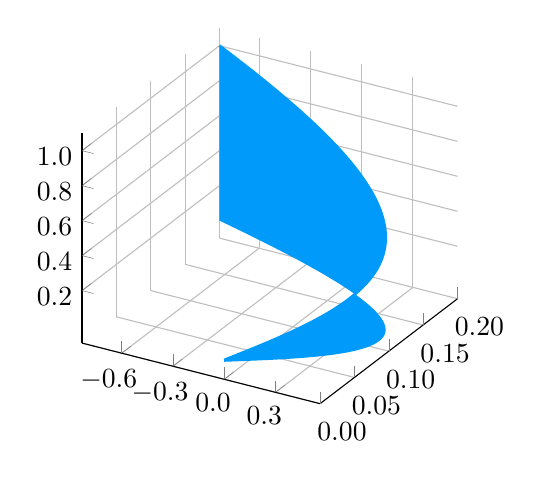
\begin{tikzpicture}[]
\begin{axis}[height = {63.5mm}, ylabel = {}, zlabel = {}, xmin = {-0.8322936730942848}, xmax = {0.5610237409422341}, ymax = {0.2}, xlabel = {}, unbounded coords=jump,scaled x ticks = false,xticklabel style={rotate = 0},xmajorgrids = true,xtick = {-0.6000000000000001,-0.30000000000000004,0.0,0.30000000000000004},xticklabels = {$-0.6$,$-0.3$,$0.0$,$0.3$},xtick align = inside,axis lines* = left,scaled y ticks = false,yticklabel style={rotate = 0},ymajorgrids = true,ytick = {0.0,0.05,0.1,0.15000000000000002,0.2},yticklabels = {$0.00$,$0.05$,$0.10$,$0.15$,$0.20$},ytick align = inside,axis lines* = left,scaled z ticks = false,zticklabel style={rotate = 0},zmajorgrids = true,ztick = {0.2,0.4,0.6000000000000001,0.8,1.0},zticklabels = {$0.2$,$0.4$,$0.6$,$0.8$,$1.0$},ztick align = inside,axis lines* = left,    xshift = 0.0mm,
    yshift = 0.0mm,
    axis background/.style={fill={rgb,1:red,1.00000000;green,1.00000000;blue,1.00000000}}
, view = {{30}{30}}, ymin = {0.0}, width = {63.5mm}]\addplot3+ [line width = 0,draw opacity = 0,fill = {rgb,1:red,0.00000000;green,0.60560316;blue,0.97868012}, fill opacity=1.0,mark = none,
mark size = 2.0,
mark options = {
    color = {rgb,1:red,0.00000000;green,0.00000000;blue,0.00000000}, draw opacity = 1.0,
    fill = {rgb,1:red,0.00000000;green,0.60560316;blue,0.97868012}, fill opacity = 1.0,
    line width = 1,
    rotate = 0,
    solid
},forget plot]coordinates {
(0.0, 0.0, 0.01)
(0.020197897901614543, 0.00202020202020202, 0.02)
(0.04037106536548054, 0.00404040404040404, 0.03)
(0.06049478877521673, 0.006060606060606061, 0.04)
(0.08054438814756551, 0.00808080808080808, 0.05)
(0.10049523392493234, 0.010101010101010102, 0.06)
(0.1203227637391126, 0.012121212121212121, 0.07)
(0.1400024991366248, 0.014141414141414142, 0.08)
(0.1595100622560901, 0.01616161616161616, 0.09)
(0.17882119244812203, 0.018181818181818184, 0.1)
(0.19791176282822218, 0.020202020202020204, 0.11)
(0.21675779675321055, 0.022222222222222223, 0.12)
(0.23533548421176181, 0.024242424242424242, 0.13)
(0.2536211981196617, 0.026262626262626265, 0.14)
(0.2715915105104493, 0.028282828282828285, 0.15)
(0.2892232086121651, 0.030303030303030304, 0.16)
(0.30649331080098463, 0.03232323232323232, 0.17)
(0.3233790824225822, 0.03434343434343434, 0.18)
(0.3398580514721388, 0.03636363636363637, 0.19)
(0.355908024123983, 0.03838383838383839, 0.2)
(0.37150710010193033, 0.04040404040404041, 0.21)
(0.3866336878814741, 0.04242424242424243, 0.22)
(0.40126651971506605, 0.044444444444444446, 0.23)
(0.4153846664718182, 0.046464646464646465, 0.24)
(0.42896755228305766, 0.048484848484848485, 0.25)
(0.4419949689852643, 0.05050505050505051, 0.26)
(0.45444709035203107, 0.05252525252525253, 0.27)
(0.4663044861067951, 0.05454545454545455, 0.28)
(0.477548135708206, 0.05656565656565657, 0.29)
(0.48815944190011357, 0.05858585858585859, 0.3)
(0.49812024401828486, 0.06060606060606061, 0.31)
(0.5074128310460859, 0.06262626262626263, 0.32)
(0.516019954411497, 0.06464646464646465, 0.33)
(0.5239248405179653, 0.06666666666666667, 0.34)
(0.5311112030017422, 0.06868686868686869, 0.35)
(0.5375632547084904, 0.0707070707070707, 0.36)
(0.5432657193821014, 0.07272727272727274, 0.37)
(0.5482038430588112, 0.07474747474747476, 0.38)
(0.5523634051598567, 0.07676767676767678, 0.39)
(0.5557307292760784, 0.0787878787878788, 0.4)
(0.5582926936380342, 0.08080808080808081, 0.41)
(0.5600367412653571, 0.08282828282828283, 0.42)
(0.5609508897892552, 0.08484848484848485, 0.43)
(0.5610237409422341, 0.08686868686868687, 0.44)
(0.5602444897092845, 0.08888888888888889, 0.45)
(0.5586029331349703, 0.09090909090909091, 0.46)
(0.5560894787810239, 0.09292929292929293, 0.47)
(0.5526951528292473, 0.09494949494949495, 0.48)
(0.5484116078247022, 0.09696969696969697, 0.49)
(0.543231130054364, 0.09898989898989899, 0.5)
(0.5371466465566053, 0.10101010101010102, 0.51)
(0.5301517317570763, 0.10303030303030304, 0.52)
(0.5222406137267401, 0.10505050505050506, 0.53)
(0.5134081800580269, 0.10707070707070708, 0.54)
(0.5036499833552723, 0.1090909090909091, 0.55)
(0.4929622463358095, 0.11111111111111112, 0.56)
(0.4813418665382922, 0.11313131313131314, 0.57)
(0.46878642063503473, 0.11515151515151516, 0.58)
(0.45529416834536657, 0.11717171717171718, 0.59)
(0.4408640559472096, 0.1191919191919192, 0.6)
(0.4254957193843033, 0.12121212121212122, 0.61)
(0.40918948696671636, 0.12323232323232323, 0.62)
(0.39194638166250045, 0.12525252525252525, 0.63)
(0.37376812297856293, 0.1272727272727273, 0.64)
(0.3546571284290503, 0.1292929292929293, 0.65)
(0.3346165145897608, 0.13131313131313133, 0.66)
(0.3136500977373192, 0.13333333333333333, 0.67)
(0.2917623940720754, 0.13535353535353536, 0.68)
(0.26895861952391015, 0.13737373737373737, 0.69)
(0.24524468914035003, 0.1393939393939394, 0.7)
(0.22062721605662822, 0.1414141414141414, 0.71)
(0.1951135100475406, 0.14343434343434344, 0.72)
(0.16871157566118242, 0.14545454545454548, 0.73)
(0.1414301099348703, 0.14747474747474748, 0.74)
(0.11327849969377658, 0.14949494949494951, 0.75)
(0.08426681843304051, 0.15151515151515152, 0.76)
(0.05440582278432834, 0.15353535353535355, 0.77)
(0.02370694856805635, 0.15555555555555556, 0.78)
(-0.00781769356729533, 0.1575757575757576, 0.79)
(-0.04015532291712722, 0.1595959595959596, 0.8)
(-0.07329249390203675, 0.16161616161616163, 0.81)
(-0.10721510165641662, 0.16363636363636364, 0.82)
(-0.14190838802200192, 0.16565656565656567, 0.83)
(-0.1773569479438341, 0.16767676767676767, 0.84)
(-0.21354473626587067, 0.1696969696969697, 0.85)
(-0.25045507492326263, 0.17171717171717174, 0.86)
(-0.28807066052810615, 0.17373737373737375, 0.87)
(-0.3263735723452442, 0.17575757575757578, 0.88)
(-0.3653452806545028, 0.17777777777777778, 0.89)
(-0.40496665549551014, 0.17979797979797982, 0.9)
(-0.44521797579105254, 0.18181818181818182, 0.91)
(-0.48607893884470893, 0.18383838383838386, 0.92)
(-0.5275286702082878, 0.18585858585858586, 0.93)
(-0.5695457339144062, 0.1878787878787879, 0.94)
(-0.6121081430693226, 0.1898989898989899, 0.95)
(-0.6551933708009587, 0.19191919191919193, 0.96)
(-0.6987783615568303, 0.19393939393939394, 0.97)
(-0.7428395427464152, 0.19595959595959597, 0.98)
(-0.787352836722307, 0.19797979797979798, 0.99)
(-0.8322936730942848, 0.2, 1.0)
(-0.8322936730942848, 0.2, 0.0)
(-0.787352836722307, 0.19797979797979798, 0.0)
(-0.7428395427464152, 0.19595959595959597, 0.0)
(-0.6987783615568303, 0.19393939393939394, 0.0)
(-0.6551933708009587, 0.19191919191919193, 0.0)
(-0.6121081430693226, 0.1898989898989899, 0.0)
(-0.5695457339144062, 0.1878787878787879, 0.0)
(-0.5275286702082878, 0.18585858585858586, 0.0)
(-0.48607893884470893, 0.18383838383838386, 0.0)
(-0.44521797579105254, 0.18181818181818182, 0.0)
(-0.40496665549551014, 0.17979797979797982, 0.0)
(-0.3653452806545028, 0.17777777777777778, 0.0)
(-0.3263735723452442, 0.17575757575757578, 0.0)
(-0.28807066052810615, 0.17373737373737375, 0.0)
(-0.25045507492326263, 0.17171717171717174, 0.0)
(-0.21354473626587067, 0.1696969696969697, 0.0)
(-0.1773569479438341, 0.16767676767676767, 0.0)
(-0.14190838802200192, 0.16565656565656567, 0.0)
(-0.10721510165641662, 0.16363636363636364, 0.0)
(-0.07329249390203675, 0.16161616161616163, 0.0)
(-0.04015532291712722, 0.1595959595959596, 0.0)
(-0.00781769356729533, 0.1575757575757576, 0.0)
(0.02370694856805635, 0.15555555555555556, 0.0)
(0.05440582278432834, 0.15353535353535355, 0.0)
(0.08426681843304051, 0.15151515151515152, 0.0)
(0.11327849969377658, 0.14949494949494951, 0.0)
(0.1414301099348703, 0.14747474747474748, 0.0)
(0.16871157566118242, 0.14545454545454548, 0.0)
(0.1951135100475406, 0.14343434343434344, 0.0)
(0.22062721605662822, 0.1414141414141414, 0.0)
(0.24524468914035003, 0.1393939393939394, 0.0)
(0.26895861952391015, 0.13737373737373737, 0.0)
(0.2917623940720754, 0.13535353535353536, 0.0)
(0.3136500977373192, 0.13333333333333333, 0.0)
(0.3346165145897608, 0.13131313131313133, 0.0)
(0.3546571284290503, 0.1292929292929293, 0.0)
(0.37376812297856293, 0.1272727272727273, 0.0)
(0.39194638166250045, 0.12525252525252525, 0.0)
(0.40918948696671636, 0.12323232323232323, 0.0)
(0.4254957193843033, 0.12121212121212122, 0.0)
(0.4408640559472096, 0.1191919191919192, 0.0)
(0.45529416834536657, 0.11717171717171718, 0.0)
(0.46878642063503473, 0.11515151515151516, 0.0)
(0.4813418665382922, 0.11313131313131314, 0.0)
(0.4929622463358095, 0.11111111111111112, 0.0)
(0.5036499833552723, 0.1090909090909091, 0.0)
(0.5134081800580269, 0.10707070707070708, 0.0)
(0.5222406137267401, 0.10505050505050506, 0.0)
(0.5301517317570763, 0.10303030303030304, 0.0)
(0.5371466465566053, 0.10101010101010102, 0.0)
(0.543231130054364, 0.09898989898989899, 0.0)
(0.5484116078247022, 0.09696969696969697, 0.0)
(0.5526951528292473, 0.09494949494949495, 0.0)
(0.5560894787810239, 0.09292929292929293, 0.0)
(0.5586029331349703, 0.09090909090909091, 0.0)
(0.5602444897092845, 0.08888888888888889, 0.0)
(0.5610237409422341, 0.08686868686868687, 0.0)
(0.5609508897892552, 0.08484848484848485, 0.0)
(0.5600367412653571, 0.08282828282828283, 0.0)
(0.5582926936380342, 0.08080808080808081, 0.0)
(0.5557307292760784, 0.0787878787878788, 0.0)
(0.5523634051598567, 0.07676767676767678, 0.0)
(0.5482038430588112, 0.07474747474747476, 0.0)
(0.5432657193821014, 0.07272727272727274, 0.0)
(0.5375632547084904, 0.0707070707070707, 0.0)
(0.5311112030017422, 0.06868686868686869, 0.0)
(0.5239248405179653, 0.06666666666666667, 0.0)
(0.516019954411497, 0.06464646464646465, 0.0)
(0.5074128310460859, 0.06262626262626263, 0.0)
(0.49812024401828486, 0.06060606060606061, 0.0)
(0.48815944190011357, 0.05858585858585859, 0.0)
(0.477548135708206, 0.05656565656565657, 0.0)
(0.4663044861067951, 0.05454545454545455, 0.0)
(0.45444709035203107, 0.05252525252525253, 0.0)
(0.4419949689852643, 0.05050505050505051, 0.0)
(0.42896755228305766, 0.048484848484848485, 0.0)
(0.4153846664718182, 0.046464646464646465, 0.0)
(0.40126651971506605, 0.044444444444444446, 0.0)
(0.3866336878814741, 0.04242424242424243, 0.0)
(0.37150710010193033, 0.04040404040404041, 0.0)
(0.355908024123983, 0.03838383838383839, 0.0)
(0.3398580514721388, 0.03636363636363637, 0.0)
(0.3233790824225822, 0.03434343434343434, 0.0)
(0.30649331080098463, 0.03232323232323232, 0.0)
(0.2892232086121651, 0.030303030303030304, 0.0)
(0.2715915105104493, 0.028282828282828285, 0.0)
(0.2536211981196617, 0.026262626262626265, 0.0)
(0.23533548421176181, 0.024242424242424242, 0.0)
(0.21675779675321055, 0.022222222222222223, 0.0)
(0.19791176282822218, 0.020202020202020204, 0.0)
(0.17882119244812203, 0.018181818181818184, 0.0)
(0.1595100622560901, 0.01616161616161616, 0.0)
(0.1400024991366248, 0.014141414141414142, 0.0)
(0.1203227637391126, 0.012121212121212121, 0.0)
(0.10049523392493234, 0.010101010101010102, 0.0)
(0.08054438814756551, 0.00808080808080808, 0.0)
(0.06049478877521673, 0.006060606060606061, 0.0)
(0.04037106536548054, 0.00404040404040404, 0.0)
(0.020197897901614543, 0.00202020202020202, 0.0)
(0.0, 0.0, 0.0)
(0.0, 0.0, 0.01)
};
\addplot3+ [color = {rgb,1:red,0.00000000;green,0.60560316;blue,0.97868012},
draw opacity=1.0,
line width=1,
solid,mark = none,
mark size = 2.0,
mark options = {
    color = {rgb,1:red,0.00000000;green,0.00000000;blue,0.00000000}, draw opacity = 1.0,
    fill = {rgb,1:red,0.00000000;green,0.60560316;blue,0.97868012}, fill opacity = 1.0,
    line width = 1,
    rotate = 0,
    solid
},forget plot]coordinates {
(0.0, 0.0, 0.01)
(0.020197897901614543, 0.00202020202020202, 0.02)
(0.04037106536548054, 0.00404040404040404, 0.03)
(0.06049478877521673, 0.006060606060606061, 0.04)
(0.08054438814756551, 0.00808080808080808, 0.05)
(0.10049523392493234, 0.010101010101010102, 0.06)
(0.1203227637391126, 0.012121212121212121, 0.07)
(0.1400024991366248, 0.014141414141414142, 0.08)
(0.1595100622560901, 0.01616161616161616, 0.09)
(0.17882119244812203, 0.018181818181818184, 0.1)
(0.19791176282822218, 0.020202020202020204, 0.11)
(0.21675779675321055, 0.022222222222222223, 0.12)
(0.23533548421176181, 0.024242424242424242, 0.13)
(0.2536211981196617, 0.026262626262626265, 0.14)
(0.2715915105104493, 0.028282828282828285, 0.15)
(0.2892232086121651, 0.030303030303030304, 0.16)
(0.30649331080098463, 0.03232323232323232, 0.17)
(0.3233790824225822, 0.03434343434343434, 0.18)
(0.3398580514721388, 0.03636363636363637, 0.19)
(0.355908024123983, 0.03838383838383839, 0.2)
(0.37150710010193033, 0.04040404040404041, 0.21)
(0.3866336878814741, 0.04242424242424243, 0.22)
(0.40126651971506605, 0.044444444444444446, 0.23)
(0.4153846664718182, 0.046464646464646465, 0.24)
(0.42896755228305766, 0.048484848484848485, 0.25)
(0.4419949689852643, 0.05050505050505051, 0.26)
(0.45444709035203107, 0.05252525252525253, 0.27)
(0.4663044861067951, 0.05454545454545455, 0.28)
(0.477548135708206, 0.05656565656565657, 0.29)
(0.48815944190011357, 0.05858585858585859, 0.3)
(0.49812024401828486, 0.06060606060606061, 0.31)
(0.5074128310460859, 0.06262626262626263, 0.32)
(0.516019954411497, 0.06464646464646465, 0.33)
(0.5239248405179653, 0.06666666666666667, 0.34)
(0.5311112030017422, 0.06868686868686869, 0.35)
(0.5375632547084904, 0.0707070707070707, 0.36)
(0.5432657193821014, 0.07272727272727274, 0.37)
(0.5482038430588112, 0.07474747474747476, 0.38)
(0.5523634051598567, 0.07676767676767678, 0.39)
(0.5557307292760784, 0.0787878787878788, 0.4)
(0.5582926936380342, 0.08080808080808081, 0.41)
(0.5600367412653571, 0.08282828282828283, 0.42)
(0.5609508897892552, 0.08484848484848485, 0.43)
(0.5610237409422341, 0.08686868686868687, 0.44)
(0.5602444897092845, 0.08888888888888889, 0.45)
(0.5586029331349703, 0.09090909090909091, 0.46)
(0.5560894787810239, 0.09292929292929293, 0.47)
(0.5526951528292473, 0.09494949494949495, 0.48)
(0.5484116078247022, 0.09696969696969697, 0.49)
(0.543231130054364, 0.09898989898989899, 0.5)
(0.5371466465566053, 0.10101010101010102, 0.51)
(0.5301517317570763, 0.10303030303030304, 0.52)
(0.5222406137267401, 0.10505050505050506, 0.53)
(0.5134081800580269, 0.10707070707070708, 0.54)
(0.5036499833552723, 0.1090909090909091, 0.55)
(0.4929622463358095, 0.11111111111111112, 0.56)
(0.4813418665382922, 0.11313131313131314, 0.57)
(0.46878642063503473, 0.11515151515151516, 0.58)
(0.45529416834536657, 0.11717171717171718, 0.59)
(0.4408640559472096, 0.1191919191919192, 0.6)
(0.4254957193843033, 0.12121212121212122, 0.61)
(0.40918948696671636, 0.12323232323232323, 0.62)
(0.39194638166250045, 0.12525252525252525, 0.63)
(0.37376812297856293, 0.1272727272727273, 0.64)
(0.3546571284290503, 0.1292929292929293, 0.65)
(0.3346165145897608, 0.13131313131313133, 0.66)
(0.3136500977373192, 0.13333333333333333, 0.67)
(0.2917623940720754, 0.13535353535353536, 0.68)
(0.26895861952391015, 0.13737373737373737, 0.69)
(0.24524468914035003, 0.1393939393939394, 0.7)
(0.22062721605662822, 0.1414141414141414, 0.71)
(0.1951135100475406, 0.14343434343434344, 0.72)
(0.16871157566118242, 0.14545454545454548, 0.73)
(0.1414301099348703, 0.14747474747474748, 0.74)
(0.11327849969377658, 0.14949494949494951, 0.75)
(0.08426681843304051, 0.15151515151515152, 0.76)
(0.05440582278432834, 0.15353535353535355, 0.77)
(0.02370694856805635, 0.15555555555555556, 0.78)
(-0.00781769356729533, 0.1575757575757576, 0.79)
(-0.04015532291712722, 0.1595959595959596, 0.8)
(-0.07329249390203675, 0.16161616161616163, 0.81)
(-0.10721510165641662, 0.16363636363636364, 0.82)
(-0.14190838802200192, 0.16565656565656567, 0.83)
(-0.1773569479438341, 0.16767676767676767, 0.84)
(-0.21354473626587067, 0.1696969696969697, 0.85)
(-0.25045507492326263, 0.17171717171717174, 0.86)
(-0.28807066052810615, 0.17373737373737375, 0.87)
(-0.3263735723452442, 0.17575757575757578, 0.88)
(-0.3653452806545028, 0.17777777777777778, 0.89)
(-0.40496665549551014, 0.17979797979797982, 0.9)
(-0.44521797579105254, 0.18181818181818182, 0.91)
(-0.48607893884470893, 0.18383838383838386, 0.92)
(-0.5275286702082878, 0.18585858585858586, 0.93)
(-0.5695457339144062, 0.1878787878787879, 0.94)
(-0.6121081430693226, 0.1898989898989899, 0.95)
(-0.6551933708009587, 0.19191919191919193, 0.96)
(-0.6987783615568303, 0.19393939393939394, 0.97)
(-0.7428395427464152, 0.19595959595959597, 0.98)
(-0.787352836722307, 0.19797979797979798, 0.99)
(-0.8322936730942848, 0.2, 1.0)
};
\end{axis}

\end{tikzpicture}

  \begin{proof}
    Since the function $f(x,y)$ is a concious function, the function $g(x,y)$
    such that $\dv{t}g(x(t),y(t)) = f(x,y)$ holds for all $t$ in real number.
    Then, we have
    \[
      \int_C f(x,y) \dd{s} = g(x_1,y_1) - g(x_0, y_0) = g(7,0) - g(2,0),
    \]
    where $(x_1,y_1)$ and $(x_0, y_0)$ are the end points of the curve $C$.
    Also, we have
    \[
      \int_2^7 f(x,0) \dd{x} = g(7, 0) - g(2, 0),
    \]
    for the right hand side of the equation. Hence $\int_C f(x,y) \dd{s} =
    \int_2^7 f(x,0) \dd{x}$ holds. This completes the proof.
  \end{proof}
\end{Answer}

\end{document}
